\documentclass[12pt,a4paper]{article}
\usepackage[utf8]{inputenc}
\usepackage[T1]{fontenc}
\usepackage{palatino}
\usepackage{amsmath}
\usepackage{amsfonts}
\usepackage{amssymb}
\usepackage{graphicx}
% Configure hyperref (must be loaded last)
\usepackage{hyperref}
\usepackage{longtable}
\usepackage[left=2.5cm,right=2.5cm,top=2.5cm,bottom=2.5cm]{geometry}
\usepackage[round,authoryear]{natbib}
\usepackage{pdflscape}         % For landscape pages
\usepackage{mdframed}          % For creating boxed environments
\usepackage{xcolor}            % For custom colors
\usepackage{tikz}             % For creating diagrams and flowcharts
\usetikzlibrary{positioning}  % For relative positioning in TikZ
\usetikzlibrary{shapes.geometric}  % For geometric shapes in TikZ
\usepackage{lineno}

% Define custom prompt environment
\definecolor{promptbg}{RGB}{250,250,250}
\definecolor{promptframe}{RGB}{200,200,200}
\newmdenv[
    linewidth=1pt,
    backgroundcolor=promptbg,
    linecolor=promptframe,
    leftmargin=1em,
    rightmargin=1em,
    innerleftmargin=1em,
    innerrightmargin=1em,
    innertopmargin=1em,
    innerbottommargin=1em,
    skipabove=1em,
    skipbelow=1em
]{prompt}





\title{Automated Diet Matrix Construction for Marine Ecosystem Models Using Generative AI}

\author{Scott Spillias\textsuperscript{1,2}\thanks{Corresponding author: scott.spillias@csiro.au} \and
Beth Fulton\textsuperscript{1,2} \and
Fabio Boschetti\textsuperscript{2,3} \and
Cathy Bulman\textsuperscript{1} \and
Joanna Strzelecki\textsuperscript{3} \and
Rowan Trebilco\textsuperscript{1,2}}

\date{\today}  % Use current date or remove for no date

\newcommand{\keywords}{%
Artificial Intelligence \and
Ecological Modeling \and
Ecopath with Ecosim \and
Large Language Models \and
Diet Interaction \and 
Large Language Models
}


% Author affiliations
\newcommand{\affiliations}{
\noindent\textsuperscript{1}CSIRO Environment, Hobart, Australia\\
\textsuperscript{2}Centre for Marine Socio-Ecology, University of Tasmania, Hobart, Australia\\
\textsuperscript{3}CSIRO Environment, IOMRC Crawley, Australia\\
\textsuperscript{4}CSIRO Environment, St. Lucia, Australia
}

\begin{document}
% \linenumbers
\maketitle
\affiliations

\begin{abstract}
This study introduces and validates a novel LLM-driven framework for automated species grouping and diet matrix generation in Ecopath with Ecosim (EwE) ecosystem models, addressing a critical bottleneck in model development. The framework uses large language models to classify marine species into functional groups and synthesize trophic interactions from diverse data sources including global biodiversity databases, species interaction repositories, and unstructured local text. We evaluate the framework across four large Australian marine regions to assess both consistency and ecological accuracy of the resulting functional groups and diet proportions. The framework demonstrated high reproducibility in species grouping decisions (>99.7\% consistency) and diet matrix construction, with 51-59\% of predator-prey interactions showing consistent diet proportions across multiple runs. Validation against expert-derived matrices for the Great Australian Bight ecosystem revealed strong ecological alignment, with the framework matching 77.6\% of functional groups and correctly identifying 85\% of trophic interactions, while estimating diet proportions within 0.2 of expert values for 80\% of interactions. These findings demonstrate the framework's potential to generate reproducible, ecologically meaningful components for ecosystem model development while significantly reducing development time.
\end{abstract}

\section{Introduction}

Ecosystem modelling is a critical tool for understanding and managing complex environments, with Ecopath with Ecosim (EwE) being a well-established framework with thousands of implementations used to model marine ecosystems and predict their responses to external pressures \citep{Christensen2004, Colleter2015}. EwE models provide quantitative insights into ecosystem structure and function, enabling researchers to assess cumulative impacts of multiple stressors and support ecosystem-based fisheries management (EBFM) decisions \citep{Coll2015, Villasante2016,Geary2020}. However, constructing these models presents significant challenges, particularly in constructing and parameterizing diet matrices that capture the complex web of trophic interactions within an ecosystem.

Traditional approaches to EwE model development rely heavily on extensive literature review, data collation and expert knowledge, which are time-consuming and resource-intensive \citep{Holden2024a}. The process of assembling diet matrices is particularly challenging, requiring synthesis of diverse data sources including field studies, literature reviews, and expert opinion. This creates a significant bottleneck in model development, especially when applying models to new geographical contexts \citep{Holden2024b}. Recent advances in artificial intelligence (AI) offer new opportunities to streamline the model development process and avoid such bottlenecks \citep{spilliasfuture}. AI tools have demonstrated success in both knowledge/evidence synthesis tasks \citep{spillias2024human,keck2025extracting,castro2024large,spillias2024evaluating,Zheng2023,nugraha2024traditional}, ecological and environmental tasks \citep{Fernandes2024,Li2024,Chen2024,dorm2025large,Noleto2024} and modelling tasks \citep{Lapeyrolerie2022, Tuia2022, Karniadakis2021}, but their application to process-based ecosystem modelling remains nascent. The key challenge lies in ensuring that AI-driven approaches can effectively synthesise available information while maintaining ecological validity.

We present a novel and flexible framework for assembling and synthesizing user-defined and online resources to parameterise EwE diet matrices using Large Language Models (LLMs). Our approach integrates multiple data sources, including global biodiversity databases, species interaction repositories, and locally-held unstructured or structured text, to automate key steps in model development. The framework employs user-selected LLMs to group species into functional units and estimate trophic interaction strengths. We evaluate the system in four distinct Australian marine ecosystems - the Northern Australia, South East shelf, and South East offshore regions, where we assess the reproducibility of the approach, and in the Great Australian Bight where we assess the accuracy of the approach. Specifically, we test the precision (repeatability) and scientific accuracy of automated species grouping decisions, and the precision and accuracy of the resulting diet matrix proportions, with accuracy defined in terms of similarity to expert estimates. These regions offer contrasting environmental conditions, species assemblages, and ecological dynamics, providing a robust test of the framework's adaptability and reliability.



\section{Methods}

\subsection{AI-Assisted Framework Overview}

The development of ecosystem models requires substantial time organizing species into functional groups and determining their interactions. This framework automates these tasks through a five-stage process that integrates artificial intelligence with ecological databases (Figure~\ref{fig:framework_overview}).

The first step in the process is to define a model domain and the resultant shapefile is used to derive a comprehensive species list from Ocean Biodiversity Information System (OBIS) \citep{Grassle1999}. In Stage 2, this species list is enriched with ecological data from FishBase and SeaLifeBase \citep{froese2010fishbase}, which provide life history traits, ecological parameters, and diet information, and with trophic interactions from the Global Biotic Interactions (GLOBI) database \citep{Poelen2014}.

Stage 3 employs a LLM for species grouping. We use Claude Sonnet-3.5 (hereafter referred to as `Claude')\citep{Anthropic2024}, though other LLMs can be incorporated. The grouping process considers both the research focus specified by the user and a generic grouping template, assigning species into functional groups.

\begin{figure}[htbp]
    \centering
    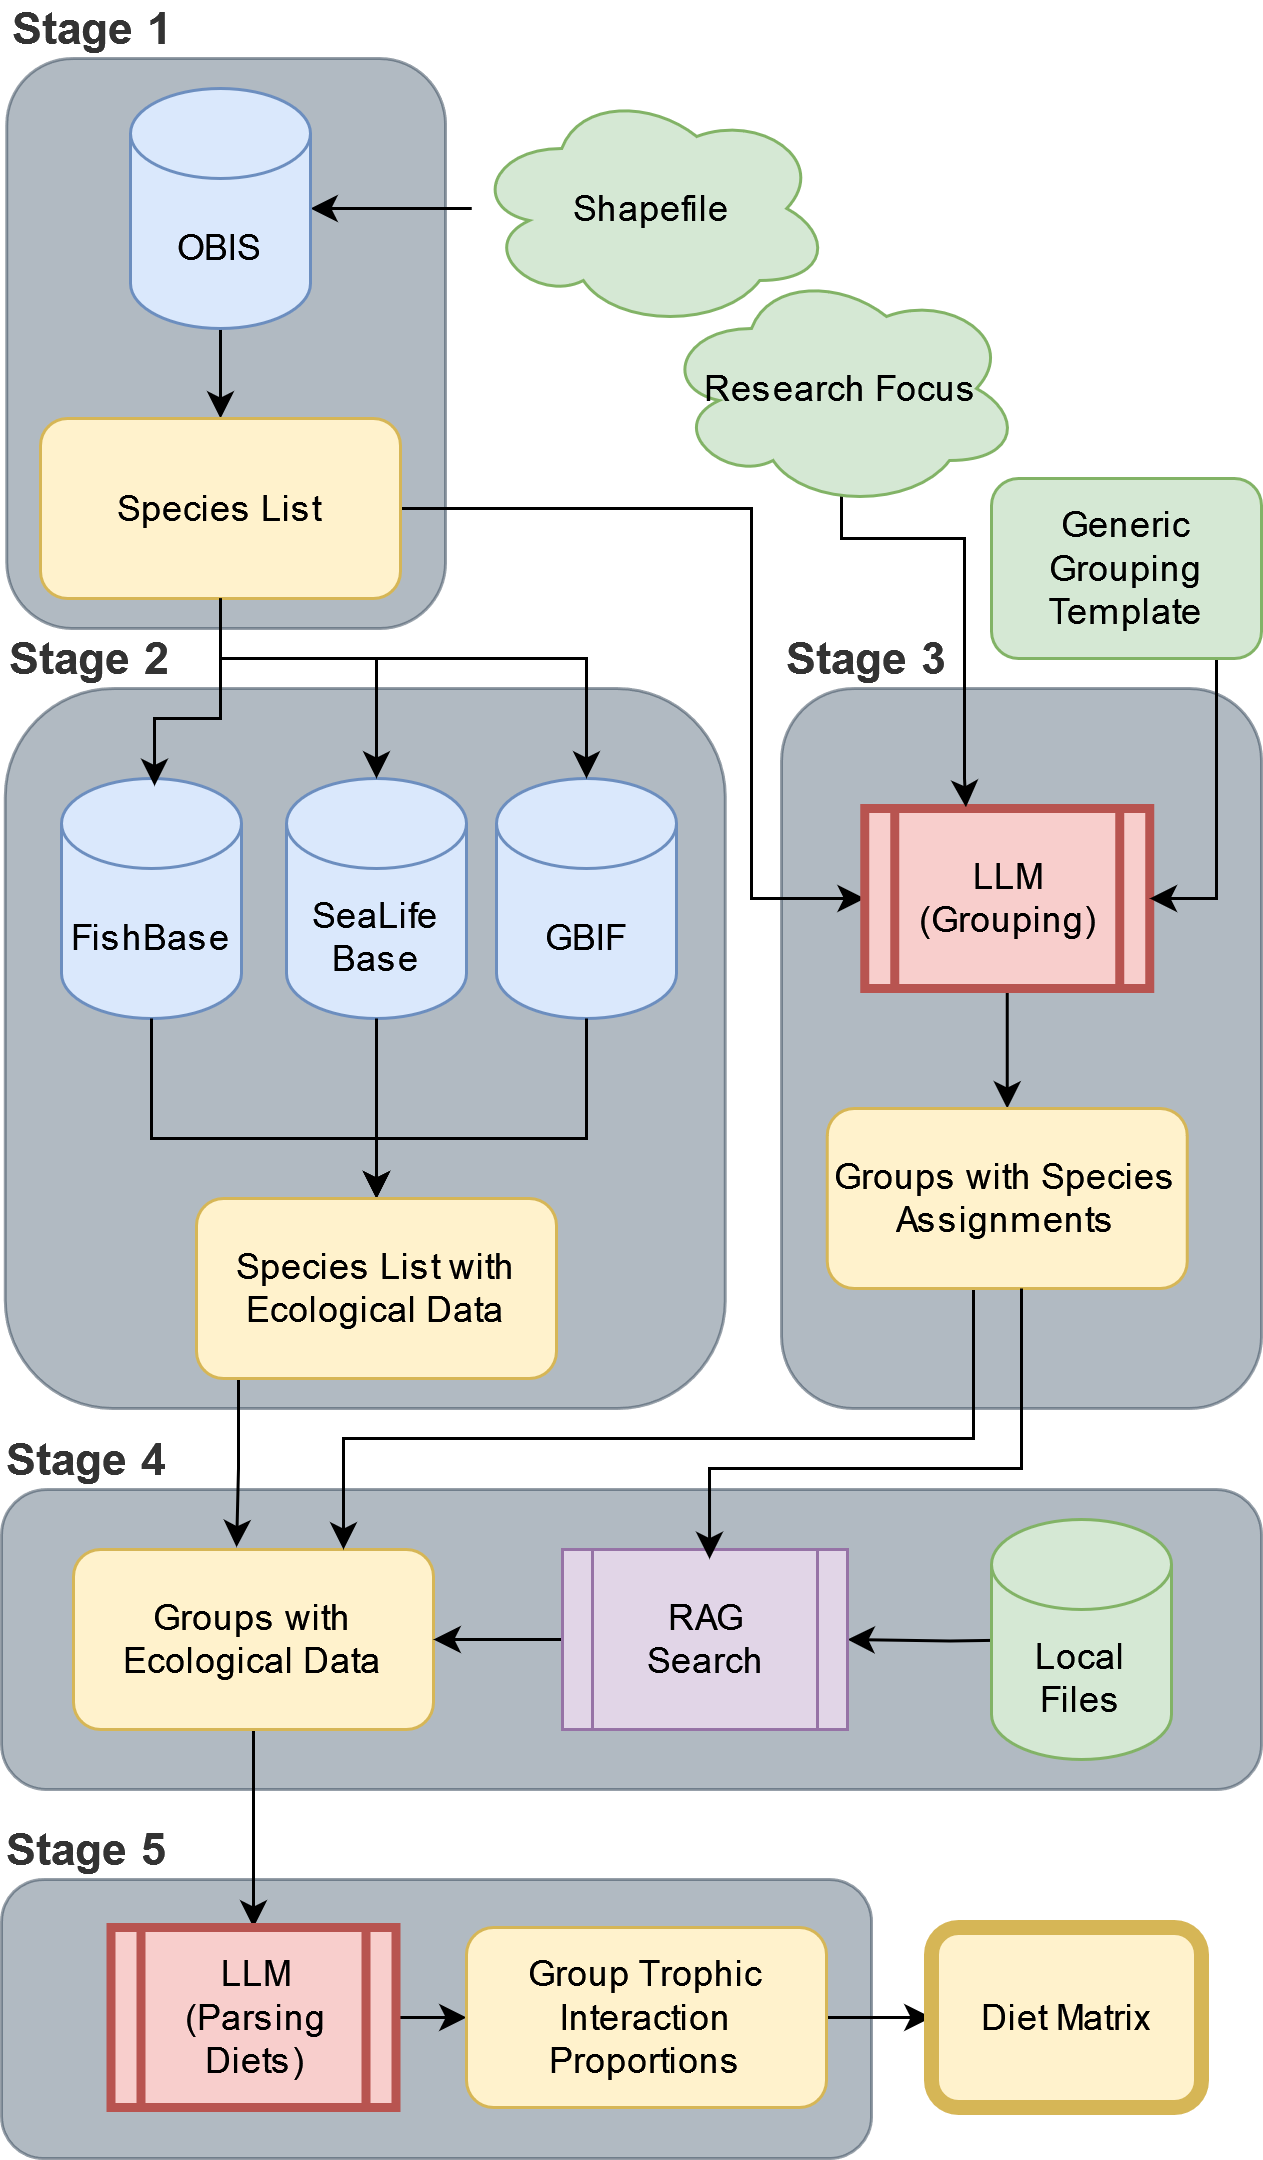
\includegraphics[width=0.5\textwidth]{figures/EwE_AI.drawio.png}
    \caption{Overview of the AI-assisted framework for ecosystem model development. The process consists of five stages: species identification, ecological data collection, functional group organization, diet data synthesis, and diet matrix construction. Each stage integrates multiple data sources and analytical approaches, with user-provided inputs (shown in green) guiding key decisions.}
    \label{fig:framework_overview}
\end{figure}

Stage 4 uses a retrieval augmented generation (RAG) system (e.g. \citep{keck2025extracting}) to synthesize the species-level ecological data into group-level summaries and incorporates user-provided local knowledge from a vector storage database, Chroma \citep{Chroma2024}, to produce group-level diet composition estimates. Finally, Stage 5 uses the LLM to parse and structure this combined data into a diet matrix, determining trophic interaction proportions among functional groups.

Section~\ref{supp:4} of the supplementary material contains detailed documentation of all processing steps, including database queries, literature search criteria, and ecological classification rules. The complete codebase and configuration files reside at [GitHub repository URL].

\subsubsection{Species Identification}

The framework begins by taking a user-defined shape file that defines the study region boundaries. It then accesses the Ocean Biodiversity Information System \citep{Grassle1999} through the \texttt{robis} R package \citep{robis}, which enables automated querying and data processing. We chose OBIS as our primary data source due to its extensive marine species coverage and standardized taxonomic classifications. 

The framework uses the `checklist' function from \texttt{robis} to retrieve scientific names and complete taxonomic classifications from kingdom to species level for all recorded species within these boundaries. Whilst collecting all occurrences would help with estimating distributions and biomasses for other modelling purposes, the time and computational resources required to process such large datasets are prohibitive and so we focus on presence only. 

To limit the amount of processing required by the LLM, the raw OBIS data is transformed in two steps. First, it filters the dataset using OBIS's \texttt{is\_marine} flag to eliminate terrestrial species that may occur in coastal records. Second, it removes taxonomic redundancy using a rank-based approach that retains only the most specific classification level available. For example, if our dataset contains both \textit{Chrysophrys auratus} (species-level) and \textit{Chrysophrys} (genus-level) entries for the same organism, our algorithm retains only the species-level entry. Our approach processes taxonomic ranks from most specific (scientific name) to most general (kingdom), keeping only the entry with the highest taxonomic resolution for each organism. 

The final species list is stored in a structured CSV file containing verified marine species and their complete taxonomic hierarchies. The complete R implementation, including rank-based filtering algorithms and geographic processing functions, is available in the project repository.

\subsubsection{Data Harvesting}

Following species identification, the framework gathers ecological and life history information for each identified species. From SeaLifeBase and FishBase \citep{froese2010fishbase}, it extracts a range of information, including habitat preferences (marine, brackish, or freshwater), depth range distributions, maximum body lengths, and ecological importance classifications. These databases are accessed through their publicly available PARQUET files using DuckDB for efficient querying of large datasets. 

Our species filtering protocol implements specific constraints to align with Ecopath with Ecosim modelling requirements. When processing taxonomic data, we prioritize species-level entries over genus-level classifications, only defaulting to genus-level when species-specific data is unavailable. For diet composition data, we extract food items including prey species codes, food groups, and prey stages. We specifically filter for adult life stages, as juvenile and larval stages are typically incorporated into planktonic functional groups rather than treated as separate components of adult diets.

We supplement the base biological data with interaction information from the Global Biotic Interactions (GLOBI) database \citep{Poelen2014}. For each species, we query the GLOBI API using URL-encoded species names to retrieve interaction records in CSV format. The GLOBI data processing preserves the raw interaction data and treats directional relationships ('eats'/'preysOn' and 'eatenBy'/'preyedUponBy') as complementary evidence of trophic interactions. For each predator-prey group pair, we tally the total number of observed interactions, which provides information about the relative frequency of feeding relationships between groups. We further enrich this data through retrieval-augmented generation (RAG) searches of regional literature (detailed in Section~\ref{supp:4.2} of the supplementary material), focusing on specific feeding relationships and dietary preferences.

Technical implementation details are provided in Section~\ref{supp:1} of the supplementary material.

\subsubsection{Species Grouping}

We implemented a template-based approach to control the quality of functional groups that are defined by the LLM. The framework uses a user-defined grouping template (provided in Section~\ref{supp:4} of the supplementary material) that leverages ecosystem modelling experience while allowing for regional customization. Due to the complexity of defining ecological groups for EwE models, we have implemented additional template-generation options but do not use them for validation in this study (See the code repository for more details).

Because OBIS can return thousands of species for a given region, instead of using an LLM to classify each species individually, which is time- and cost-prohibitive, we group species hierarchically to reduce the number of classifications required. The framework does this iteratively traversing the resulting OBIS database, from kingdom to species, classifying taxonomic groups into functional groups at finer and finer resolutions. Starting at the Kingdom level, the LLM is asked to classify taxa into functional groups. Taxa that the LLM does not think fall neatly into a specific functional group undergo evaluation at finer taxonomic levels until reaching a definitive group assignment or the species level. 

For example, when classifying something like the Western Australian Dhufish (Glaucosoma hebraicum), after passing through the Kingdom Animalia, the phylum Chordata is evaluated. Since Chordata includes diverse feeding strategies from filter-feeding tunicates to predatory fish, the LLM marks it for resolution at a finer level. At the class level, the LLM evaluates Actinopterygii, which is again marked for resolution due to its diverse feeding strategies. Continuing through the taxonomic hierarchy, the family Glaucosomatidae is eventually reached, where all members share similar ecological roles as demersal predators, allowing classification into the demersal carnivore functional group. This hierarchical approach significantly reduces the number of required classifications, although is vulnerable to misclassifications at higher taxonomic levels if the LLM does not have sufficient ecological capability. The success of this approach is highly dependent on the quality of the grouping template and the LLM's ability to understand the ecological roles of taxa and is a key target for validation in this study. We provide an initial evaluation of the quality of this LLM-generated grouping in Section~\ref{supp:3}.


At each taxonomic level, the LLM evaluates taxa against the selected grouping template using the following prompt (where square brackets indicate dynamically updated variables):

\begin{prompt}
You are classifying marine organisms into functional groups for an Ecopath with Ecosim (EwE) model. Functional groups can be individual species or groups of species that perform a similar function in the ecosystem, i.e.\ have approximately the same growth rates, consumption rates, diets, habitats, and predators. They should be based on species that occupy similar niches, rather than of similar taxonomic groups.

Examine these taxa at the [rank] level and assign each to an ecological functional group.

Rules for assignment:
\begin{itemize}
\item If a taxon contains members with different feeding strategies or trophic levels, assign it to `RESOLVE'
\item Examples requiring `RESOLVE':
  \begin{itemize}
  \item A phylum containing both filter feeders and predators
  \item An order with both herbivores and carnivores
  \item A class with species across multiple trophic levels
  \end{itemize}
\item If all members of a taxon share similar ecological roles, assign to an appropriate group
\item Only consider the adult phase of the organisms, larvae and juveniles will be organized separately
\item Only assign a definite group if you are confident ALL members of that taxon belong to that group
\end{itemize}

Taxa to classify:
[List of taxa]

Available ecological groups (name: description):
[List of available groups and their descriptions]

Return only a JSON object with taxa as keys and assigned groups as values.
\end{prompt}

When the research focus indicates areas requiring higher resolution (e.g., commercial fisheries species), we modify the classification process with additional guidance:

\begin{prompt}
Special consideration for research focus:
The model's research focus is: [research focus]

When classifying taxa that are related to this research focus:
\begin{itemize}
\item Consider creating more detailed, finer resolution groupings
\item Keep species of particular interest as individual functional groups
\item For taxa that interact significantly with the focal species/groups, maintain higher resolution groupings
\item For other taxa, broader functional groups may be appropriate
\end{itemize}
\end{prompt}

The framework maintains complete provenance information, including the source of group definitions and any AI-suggested modifications. The system automatically includes a Detritus functional group to represent non-living organic matter in the ecosystem. Finally, a detailed grouping report is produced which documents all of the classification decisions for later human review.

\subsubsection{Diet Matrix Construction}

After the framework has assigned species to groups, the species-level diet and ecological information collected in Stage 2 is re-assigned to the new functional groups. The diet matrix construction involves two LLM-driven steps. First, the framework assembles text data from various sources (RAG search results, diet data, and GLOBI interaction data) into a structured profile for each group. This profile is passed to the LLM to generate an initial diet composition summary. The following prompt guides this first LLM analysis:

\begin{prompt}
Based on the following information about the diet composition of [group], provide a summary of their diet. Include the prey items and their estimated proportions in the diet.

Available functional groups and their details:
[List of groups with descriptions and top species]

Here is the diet data for [group]:
[Combined data including RAG search results, compressed food categories, and GLOBI interactions]

Format your response as a list, with each item on a new line in the following format:

Prey Item: Percentage

For example:
\begin{verbatim}
Small fish: 40%
Zooplankton: 30%
Algae: 20%
Detritus: 10%
\end{verbatim}

If exact percentages are not available, estimate percentages based on the information you have been provided.
Ensure that all percentages add up to approximately 100\%.
Consider the RAG search results, compressed food categories, and GLOBI data when creating your summary.
Pay special attention to the GLOBI interaction counts, which indicate frequency of observed feeding relationships.
Note that some species may feed on juvenile or larval forms of other species, which are often classified in different functional groups than the adults.
\end{prompt}

Sometimes these responses contain functional groups that are not included in the list of accepted groups or do not add up to 100\%. Therefore, the initial diet summaries are passed to a second LLM step that standardizes the proportions and maps any groups from the first answer to the already-defined functional groups. This second step converts the approximate summaries into a structured diet matrix, with prey items as rows and predators as columns. Each cell contains the proportion of the predator's diet comprised of that prey item. The diet matrix is then output as a CSV file for use in Ecopath with Ecosim models. 

When prey items do not exactly match functional group names, we employ a hierarchical matching system. The system first attempts exact matches, then falls back to case-insensitive partial matching using species names. For example, if the AI returns a prey item "snapper" that doesn't exactly match any functional group, the system would match it to a functional group containing ``snapper'' in its name such as ``Pink Snapper''.

This process is the second target of validation in this study and is evaluated in Section~\ref{supp:2}. The complete codebase and configuration files are available at [GitHub repository URL].

%\subsubsection{Parameter Estimation (Likely to be removed - no validation)}

The final stage estimates the required Ecopath \citep{Christensen2004} parameters for each functional group. We query the EcoBase repository \citep{Colleter2015} using a structured search strategy that combines group names with regional context (e.g., "Western Australian shelf species in [group]"). For each functional group, we retrieve five key parameters from comparable models: habitat area fractions, biomass densities (t/km$^2$), production/biomass ratios (P/B, year$^{-1}$), consumption/biomass ratios (Q/B, year$^{-1}$), and ecotrophic efficiency (EE).

We implement parameter-specific validation checks. For biomass densities, we verify values fall within expected ranges for each functional group type. For P/B and Q/B ratios, we check consistency with known allometric relationships and life history characteristics. EE values must fall between 0 and 1, with additional validation against typical ranges for similar species groups.

Claude \citep{Anthropic2024} analyzes these parameter sets using standardized criteria. The analysis considers the relevance of each model to the group in question, the consistency of values across different models, trends or patterns in the data that might indicate suitable values, and the ecological context provided by model metadata.

For each parameter assignment, Claude provides a structured response containing the suggested parameter value, detailed reasoning for the selection, references to source models, and any assumptions or caveats.

When EcoBase data is insufficient or parameter values show high variability, we employ a hierarchical fallback system. First, we search for parameters from taxonomically similar groups. Next, we apply empirical relationships where available. Finally, if automated methods are unsuitable, we flag the parameter for manual parameterization.

The system maintains comprehensive logging of parameter assignments. This includes search queries and results, parameter validation checks, AI reasoning and decisions, source model references, and data quality assessments.

The final output consists of a structured JSON file containing the complete parameter set for each functional group. This format preserves the full provenance of each parameter value while enabling automated validation and mass-balance calculations in Ecopath.



\subsection{Framework Consistency Assessment}

Our validation framework assesses both the precision (consistency across multiple runs) and accuracy (comparison with expert-created matrices) of the LLM-driven model construction process. This dual approach provides comprehensive insights into the framework's reliability and ecological validity.

We executed model generation across three distinct phases. In phase one, we established baseline configurations for each study region by processing species occurrence data and research parameters, creating standardized input states for subsequent iterations. In phase two, we executed five independent iterations per region, maintaining fixed input parameters while allowing the LLM's stochastic decision processes to generate natural variation in outputs. In phase three, we conducted detailed statistical analyses of both consistency across iterations and accuracy compared to expert-created matrices.

For consistency assessment, we calculated group stability scores using Jaccard similarity coefficients between consecutive iterations and analysed the coefficient of variation in diet proportions. For the accuracy assessment, we averaged the diet proportions of the five LLM-generated matrices and compared the resulting matrix with an expert-created matrix for the Great Australian Bight ecosystem (C. Bulman pers. comm.) that was used to inform \citep{Fulton2018}. 

\subsubsection{Study Regions}

\begin{figure}[htbp]
    \centering
    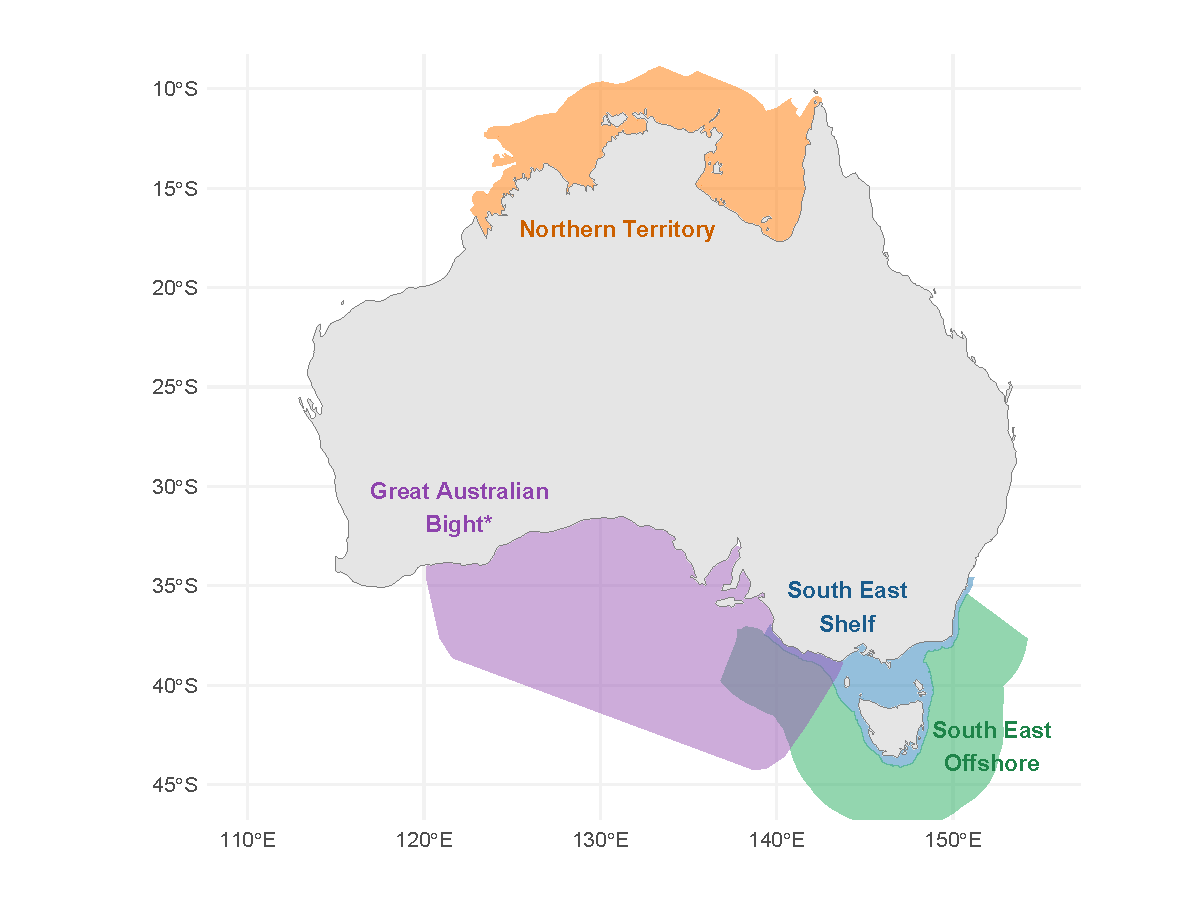
\includegraphics[width=0.8\textwidth]{figures/validation_regions.pdf}
    \caption{Map of the three study regions used for consistency assessment: Northern Territory (orange), South East shelf (blue), South East Offshore (green), and the Great Australian Bight (purple). *We used the GAB study region to test the accuracy of our approach by comparing it to the initial diet matrix used in \citep{Fulton2018}, we used the other regions to test the replicability of the approach.}
    \label{fig:validation_regions}
    \end{figure}

We assess our framework using three Australian marine regions that present distinct ecological characteristics and modelling challenges (Figure \ref{fig:validation_regions}). The Northern Territory region represents a tropical ecosystem characterised by complex reef systems, seasonal monsoon influences, and high biodiversity. This region tests the framework's ability to handle diverse species assemblages and complex trophic interactions in a dynamic environment.

The South East shelf region represents a temperate coastal system with extensive ecological records. This region has comprehensive diet information in established databases, well-documented EwE models spanning multiple years, and active research programs. The rich availability of expert knowledge and historical data makes this region ideal for assessing the framework's data integration capabilities.

The South East Offshore region presents a deep-water ecosystem that challenges the framework with data-limited conditions and unique ecological patterns. This region tests the framework's capacity to handle situations where direct observational data may be sparse and where species interactions may be less well understood. The contrasting characteristics of these three regions provide a robust test of the framework's adaptability across different ecological contexts.

\subsubsection{Species Grouping Reproducibility Analysis}

To assess the reproducibility of AI-generated species groupings, we developed quantitative measures of grouping consistency. We tracked each species' group assignments across iterations and calculated a consistency score:

\[
\text{Consistency Score} = \frac{\text{Number of occurrences in most common group}}{\text{Total number of iterations}}
\]

This metric quantifies the framework's decision-making reliability for individual species. We classified species with consistency scores below 0.95 as unstable, indicating variable group assignments across iterations. Chi-square tests on these consistency scores help identify whether grouping decisions remain stable across different ecological contexts, addressing a key aspect of the framework's reliability.

To evaluate broader patterns in group formation, we assessed group stability using the Jaccard similarity coefficient between consecutive iterations:

\[
J(i,j) = \frac{|M_{i} \cap M_{j}|}{|M_{i} \cup M_{j}|}
\]

where $M_{i}$ and $M_{j}$ represented species members in iterations $i$ and $j$. We calculated the overall stability score by averaging Jaccard similarities across consecutive iteration pairs. This approach, combined with coefficients of variation analysis, reveals how consistently the framework identifies and maintains ecologically meaningful groupings across different runs. One-way ANOVA tests on these stability measures across regions, supplemented with Cohen's f effect size calculations, demonstrate the framework's reproducibility across different marine ecosystems while maintaining consistent decision-making patterns.

\subsubsection{Diet Matrix Reproducibility Assessment}
To evaluate the consistency of AI-generated trophic interactions and assess the framework's ability to capture distinct ecological patterns, we developed a multi-metric analysis approach. We focused on significant predator-prey interactions, defined as those comprising more than 5\% of a predator's diet, using both descriptive statistics and correlation analyses. For each interaction, we calculated:

\begin{enumerate}
    \item Presence ratio across iterations:
    \[
    P_{ij} = \frac{\text{Number of iterations with interaction}}{n}
    \]
    where $n$ was the total number of iterations.

    \item Mean diet proportion:
    \[
    \mu_{ij} = \frac{1}{n}\sum_{k=1}^{n} x_{ijk}
    \]
    where $x_{ijk}$ represents diet proportion for predator $i$ consuming prey $j$ in iteration $k$.

    \item Stability score:
    \[
    S_{ij} = \frac{1}{n}\sum_{k=1}^{n} \frac{|x_{ijk} - \mu_{ij}|}{\max_{k}(x_{ijk})}
    \]
    where $x_{ijk}$ represents the diet proportion for predator $i$ consuming prey $j$ in iteration $k$, $\mu_{ij}$ is the mean diet proportion across iterations, and $\max_{k}(x_{ijk})$ is the maximum value across iterations. This score ranges from 0 (perfect stability) to 1 (maximum instability), with lower values indicating more consistent diet proportions across iterations.
\end{enumerate}

We chose this stability metric over traditional variance measures for several reasons. First, by normalizing deviations by the maximum value, the metric achieves scale independence, allowing meaningful comparisons between interactions of different magnitudes. For example, the sequences [0.2, 0.2, 0.2, 0.2, 0.1] and [0.02, 0.02, 0.02, 0.02, 0.01] would yield the same stability score despite having different absolute variances. Second, the bounded range between 0 and 1 provides an intuitive scale for assessing stability, unlike the unbounded nature of variance. Third, this approach effectively handles small variations in small values, ensuring that minor fluctuations in trace diet components do not disproportionately influence the stability assessment.

We classified interactions as unstable when their stability score exceeded 0.3, indicating significant variation in diet proportions across iterations. To illustrate this metric:

\begin{itemize}
    \item A stable interaction (S = 0.08) might show values [0.02, 0.02, 0.02, 0.02, 0.01], where proportions remain very similar across iterations
    \item An unstable interaction (S = 0.39) might show values [0.027, 0.25, 0.25, 0.067, 0.25], where proportions vary substantially between iterations
\end{itemize}

This metric provides a continuous measure of stability that handles both presence/absence patterns and magnitude variations in a unified way, avoiding discontinuities at zero values. To assess the framework's ability to capture distinct ecological patterns across regions, we employed pairwise Spearman correlations between iterations to evaluate the consistency of predator-prey relationships, focusing on significant interactions. This non-parametric approach accounts for the potentially non-normal distribution of diet proportions. We supplemented this with Kruskal-Wallis tests to identify significant differences in trophic structure across regions, providing evidence of the framework's ability to distinguish unique ecological characteristics in different marine ecosystems.

\subsubsection{Diet Matrix Accuracy Assessment}
\label{sec:accuracy_assessment}
To evaluate the accuracy of AI-generated diet matrices against expert knowledge, we conducted a detailed comparison using the Great Australian Bight (GAB) ecosystem model developed by \citet{Fulton2018}. We obtained the original, unbalanced diet matrix constructed by expert marine ecologists (C. Bulman, personal communication) and compared it with five independently generated AI matrices for the same region. We isolate the diet proportion accuracy by providing the AI system with the same list of groupings from the extant GAB model, thus testing the systems ability to sort species into the correct groups and then assign diet proportions according to those group. 

The analysis examined two fundamental aspects of the diet matrices: the structural patterns of predator-prey relationships and the quantitative diet proportions. We first assessed structural agreement by identifying matching and mismatching interactions between the expert and AI matrices. This binary presence-absence analysis yielded counts of concordant interactions, where both matrices agreed on the presence or absence of a feeding relationship, and discordant interactions where one matrix indicated a link while the other did not. We quantified the overall agreement using Cohen's Kappa coefficient, supplemented by true positive and negative rates to characterise the framework's ability to replicate expert-identified trophic relationships.

For predator-prey pairs where both matrices indicated an interaction, we conducted quantitative comparisons of the diet proportions. We calculated the Pearson correlation coefficients to measure the relationship between expert and AI-assigned proportions. We performed these analyses both at the whole-matrix level and for individual predator groups, enabling identification of systematic patterns in the framework's performance across different taxonomic groups.


\section{Results}

Our validation framework assessed three key aspects of the AI-assisted ecosystem modelling approach: reproducibility of species groupings, consistency of diet matrix construction, and accuracy against expert-derived matrices. 

\subsection{Species Grouping Reproducibility}
% Addressing Objective 2a: Assess consistency of species grouping decisions

\subsubsection{Classification Consistency Analysis}
The framework successfully reduced ecological complexity while preserving meaningful biological relationships. Starting with 63 potential functional groups provided in the default template (See \ref{supp:technical_implementation}), it identified 34-37 region-specific groups. Chi-square tests confirmed the non-random nature of these groupings, showing consistent species assignments across all regions (p < 0.001). This statistical significance provides strong evidence that the framework makes systematic grouping decisions rather than arbitrary assignments.

The framework achieved high classification stability for groups across all regions. Mean consistency scores, where 1.0 represents identical species assignments to groups across all groups and within-region iterations, were exceptionally high: 0.997 for both Northern Australia and South East shelf, and 0.998 for South East Offshore. This translated to very low proportions of species that were variably classified across the five iterations: only 0.99\% (103 species) in Northern Australia, 1.06\% (125 species) in South East shelf, and 0.73\% (87 species) in South East Offshore. These results demonstrate that the framework's classifications remained stable despite the stochastic nature of the AI decision-making process.

Among the small percentage of variably classified species, we identified consistent patterns of classification instability (Table \ref{tab:unstable_species}). These species typically oscillated between ecologically similar functional groups, such as macrozoobenthos and benthic infaunal carnivores in the Northern Australia, or piscivores and deep demersal fish in the South East Inshore region. This suggests that classification uncertainty occurs primarily at ecological boundaries where functional roles overlap.

The Jaccard similarity indices reveal high overall stability in group membership across all three regions (Figure \ref{fig:regional_analysis}), with most functional groups showing indices above 0.95. The groups labelled in the figure represent those groups with lower stability indices.

Further detailed analysis of group stability patterns across regions is provided in \ref{supp:group_stability}.

\begin{figure}[htbp]
    \centering
    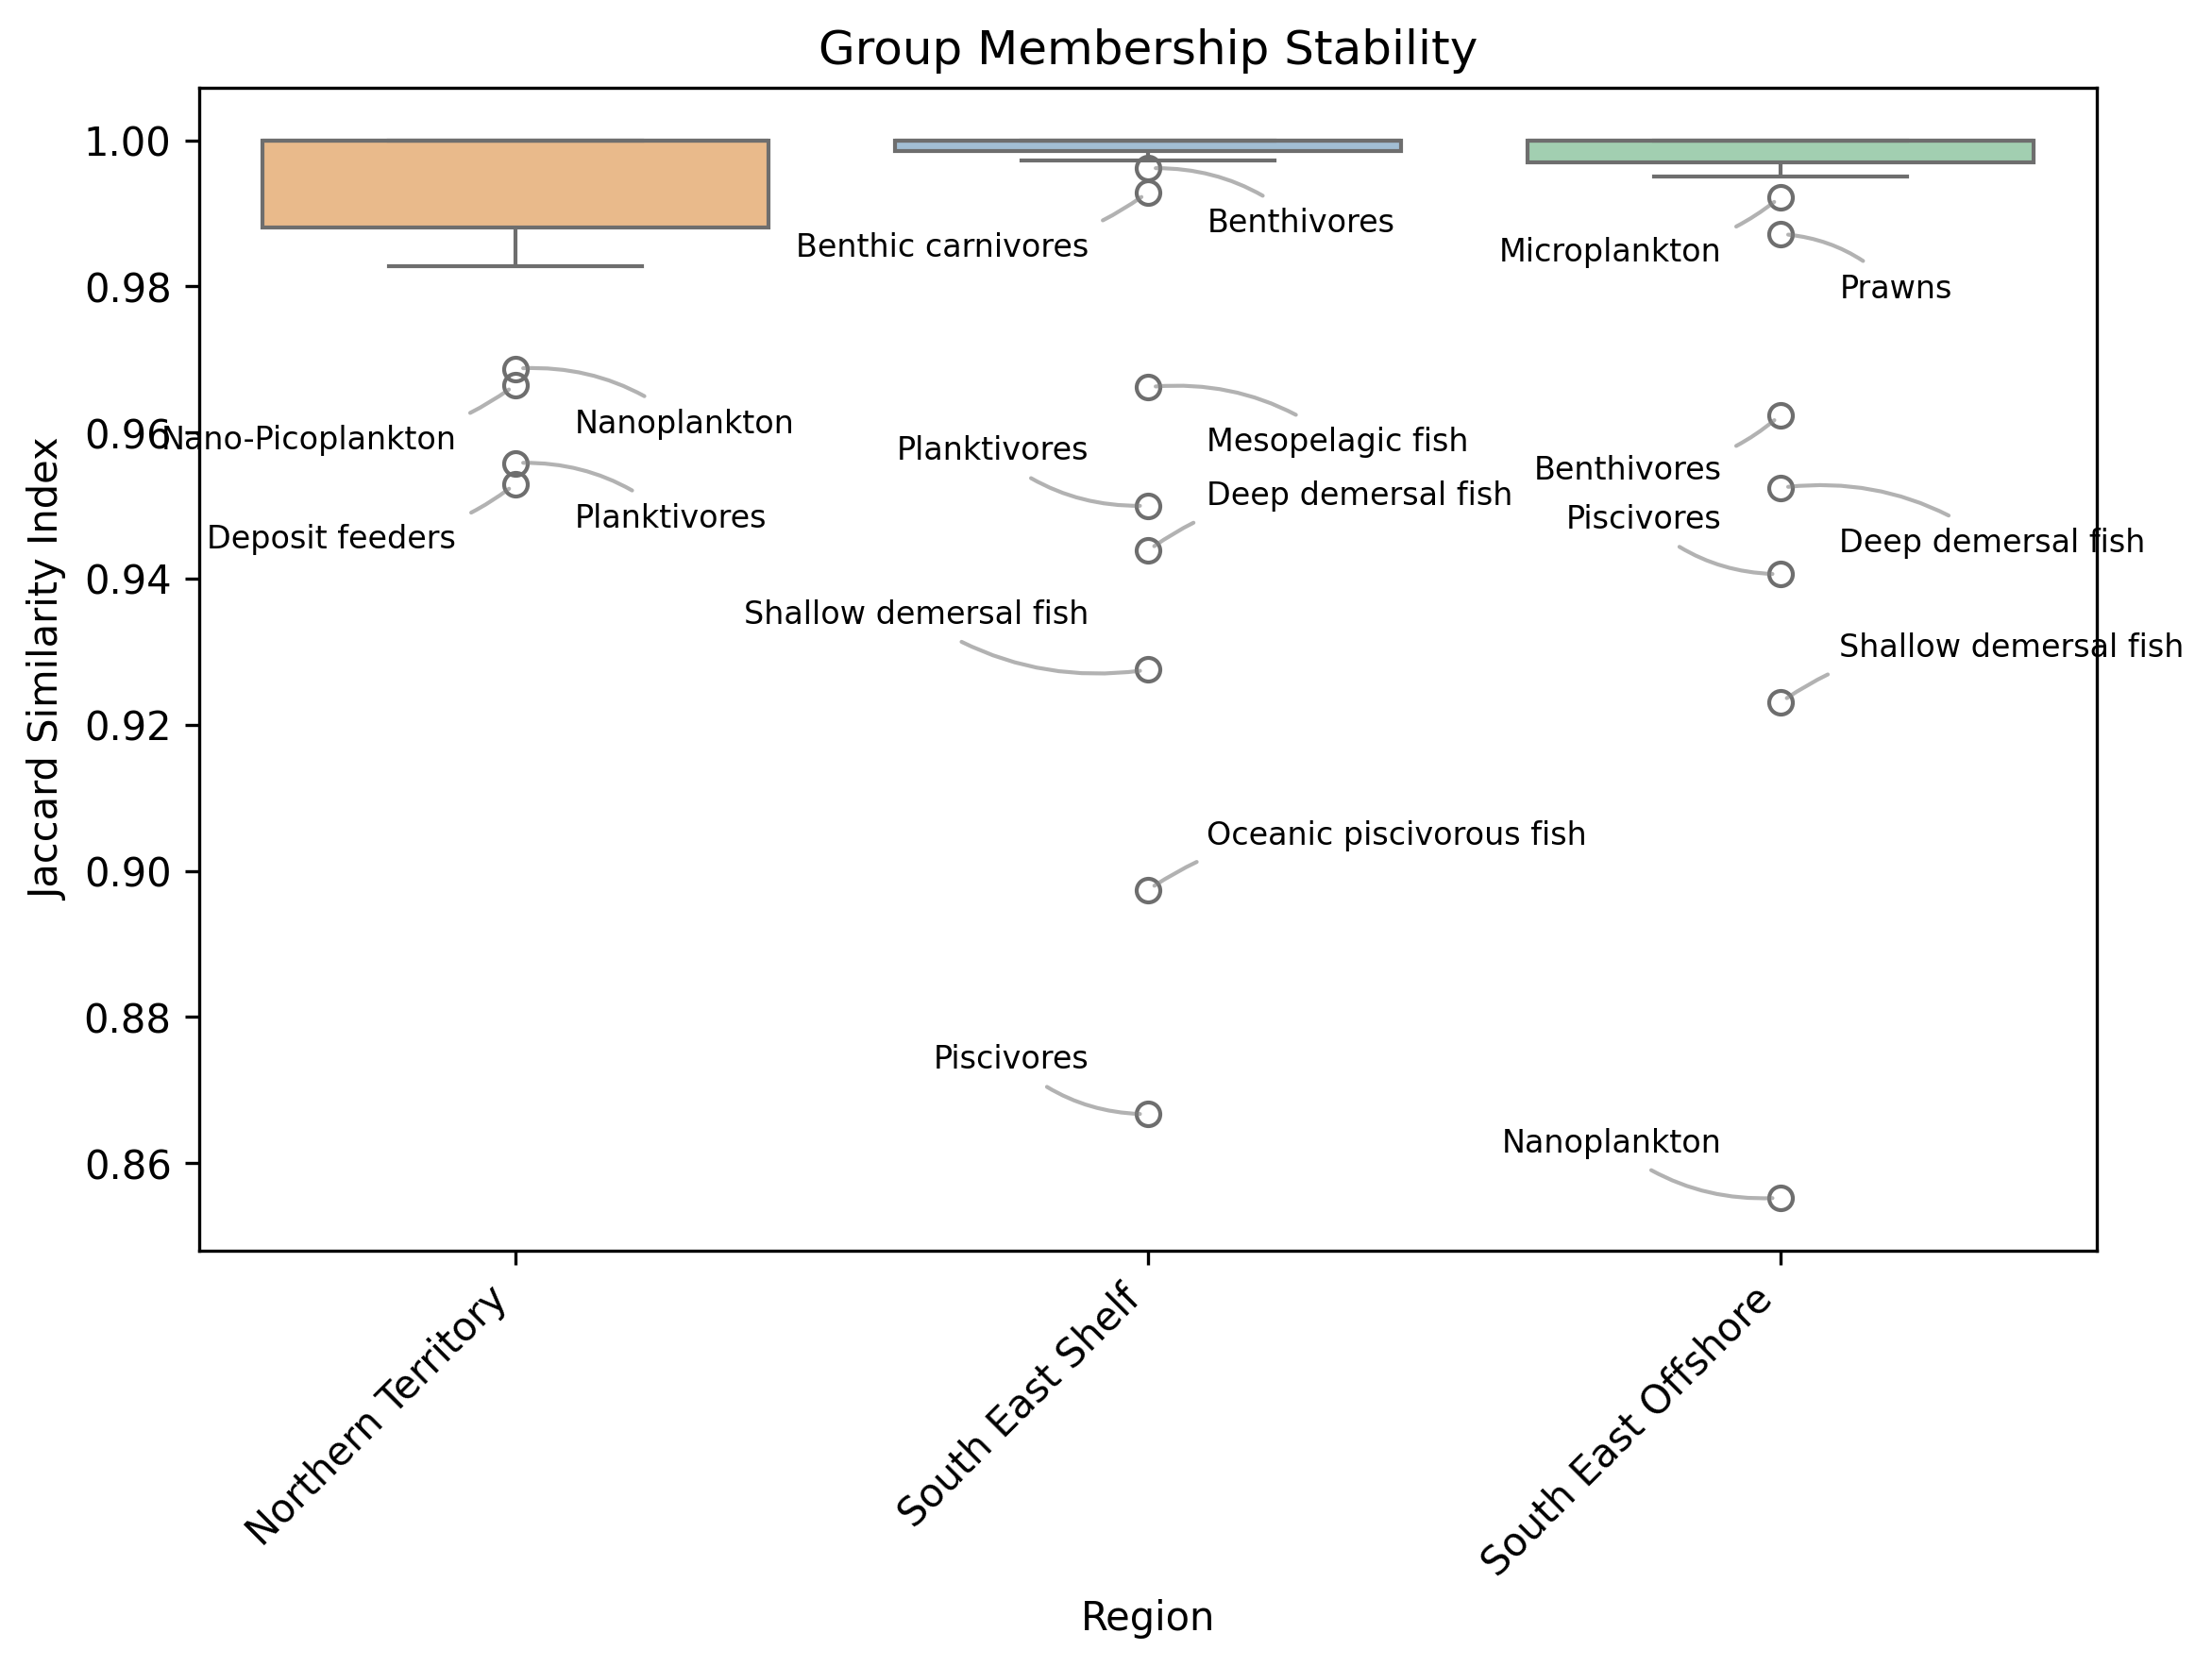
\includegraphics[width=\textwidth]{figures/regional_group_analysis.png}
    \caption{Group membership stability across three regions measured by Jaccard similarity index (0.85-1.0). Most groups show high stability (>0.95), with labelled points out-of-distribution outliers that exhibit lower stability.}
    \label{fig:regional_analysis}
\end{figure}

\begin{table}[htbp]
\centering
\caption{Dominant patterns of species classification instability across three study regions. The table presents the most frequent oscillation patterns between functional groups for species that were inconsistently classified across the five framework iterations. For each region, the total number of variably classified species is shown (representing less than 1.1\% of all species), along with the percentage distribution of different oscillation patterns.}
\label{tab:unstable_species}
\small
\begin{tabular}{llcc}
\hline
Region & Most Common Pattern & Count & \% of Total \\
\hline
Northern & Macrozoobenthos $\leftrightarrow$ Benthic infaunal carnivores & 28 & 27.2\% \\
Territory & Benthic filter feeders $\leftrightarrow$ Deposit feeders & 25 & 24.3\% \\
(103 species) & Prawns $\leftrightarrow$ Macrozoobenthos & 21 & 20.4\% \\
& Other patterns & 29 & 28.1\% \\
\hline
South East & Piscivores $\leftrightarrow$ Deep demersal fish & 42 & 33.6\% \\
Inshore & Benthic grazers $\leftrightarrow$ Benthic carnivores & 31 & 24.8\% \\
(125 species) & Planktivores $\leftrightarrow$ Mesopelagic fish & 28 & 22.4\% \\
& Other patterns & 24 & 19.2\% \\
\hline
South East & Benthic filter feeders $\leftrightarrow$ Benthic carnivores & 25 & 28.7\% \\
Offshore & Macrozoobenthos $\leftrightarrow$ Deep demersal fish & 22 & 25.3\% \\
(87 species) & Mesozooplankton $\leftrightarrow$ Macrozoobenthos & 18 & 20.7\% \\
& Other patterns & 22 & 25.3\% \\
\hline
\multicolumn{4}{p{0.95\textwidth}}{\small \textit{Note:} Arrows indicate group assignment oscillation between iterations. Complete species-level data available in Section S3 of the supplementary material.} \\
\hline
\end{tabular}
\end{table}


\subsection{Diet Matrix Reproducibility}
% Addressing Objective 2b: Assess consistency of diet matrix values

\subsubsection{Trophic Interaction Consistency}
The framework identified consistent trophic relationships across all regions, with the Northern Australia showing 358 interactions (58.7\% having stability scores > 0.7), South East shelf 380 interactions (51.3\% of which were stable), and South East Offshore 477 interactions (56.0\% stable). As shown in Figure \ref{fig:stability_distribution}, the distribution of stability scores across regions demonstrates that most interactions cluster above the 0.7 threshold, with a substantial proportion achieving near-perfect stability (scores approaching 1.0). Spearman correlations between iterations demonstrated that the relative proportions of different prey in predator diets remained fairly consistent across all regions (Northern Australia: $\rho = 0.72-0.89$; South East shelf: $\rho = 0.68-0.85$; South East Offshore: $\rho = 0.70-0.87$), even when absolute proportions varied. Detailed diet matrices for each region are provided in \ref{supp:diet_matrix}.

\begin{figure}[htbp]
    \centering
    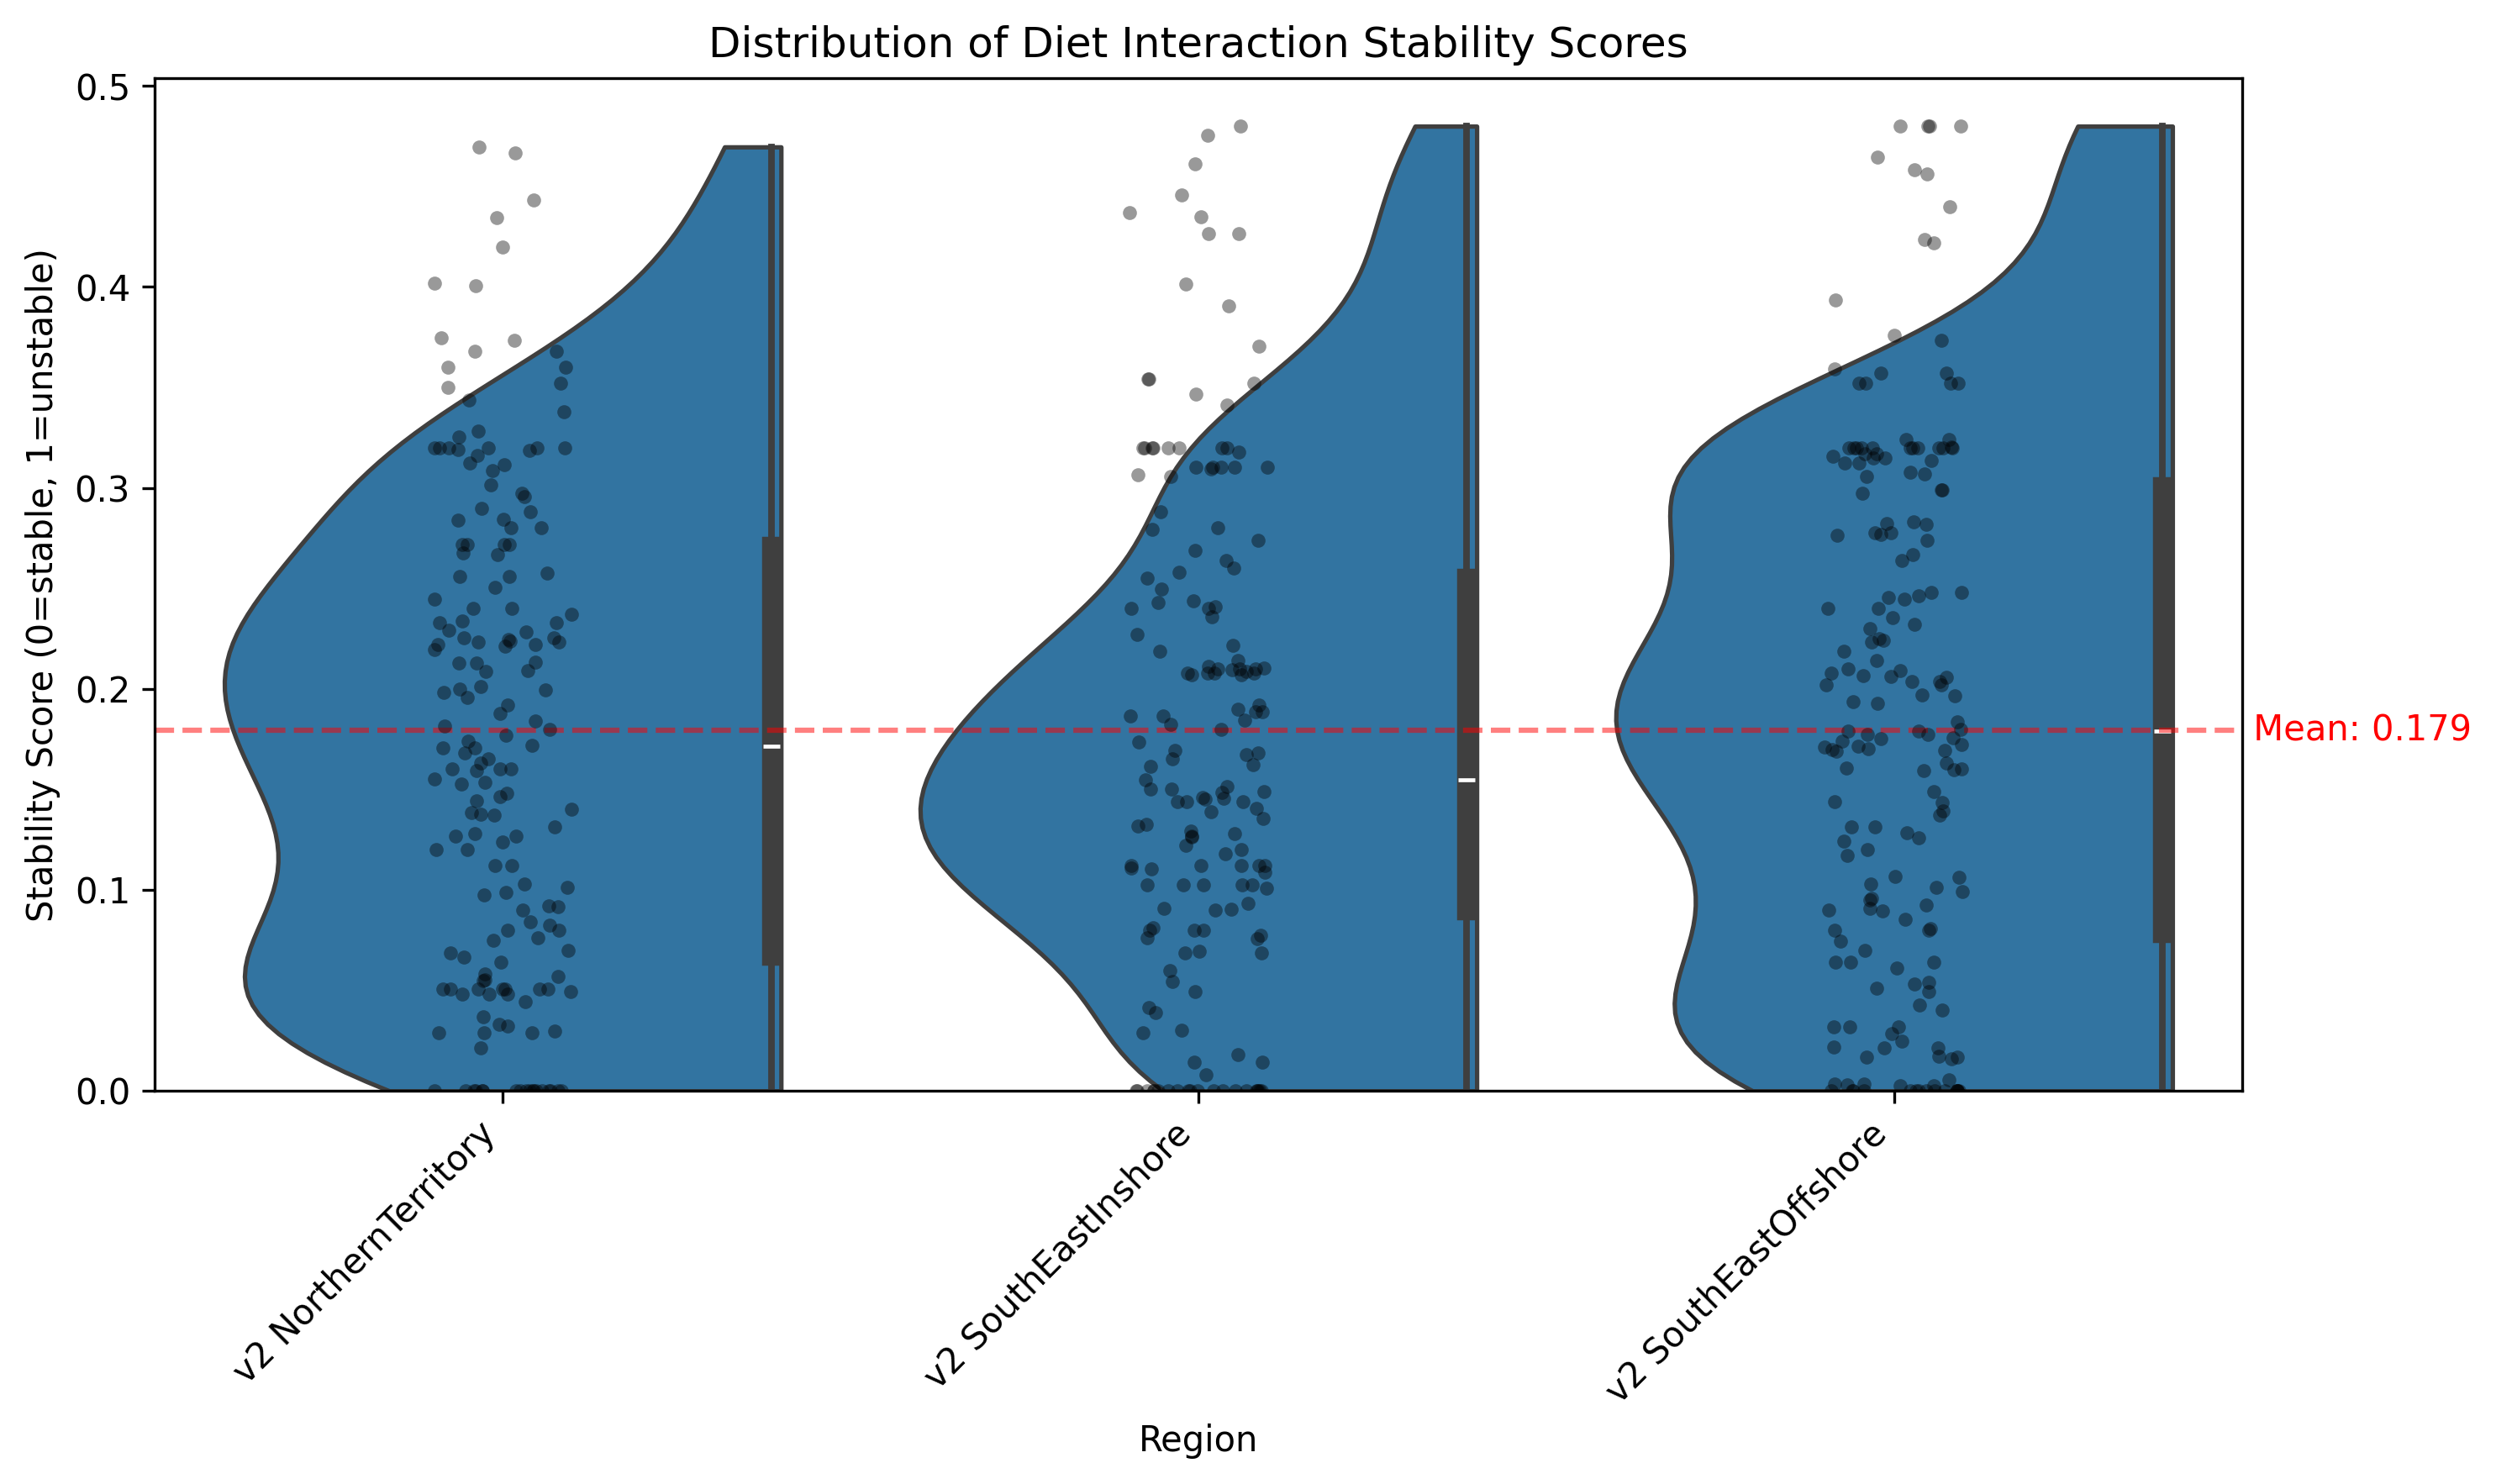
\includegraphics[width=\textwidth]{figures/stability_score_distribution.png}
    \caption{Distribution of diet interaction stability scores across regions for substantial interactions (those comprising more than 5\% of a predator's diet). Half-violin plots show the density of stability scores (1=stable, 0=unstable), with embedded box plots indicating quartiles and median. Individual points represent specific predator-prey interactions, and the red dashed line shows the mean stability score across all regions. The distributions are bounded at one, reflecting perfect stability, with most interactions showing scores above 0.7. Stability scores quantify the consistency of predator-prey interactions across iterations, where a score of 1.0 indicates the interaction was identified with identical diet proportions in all iterations, while lower scores reflect either variable diet proportions or inconsistent identification of the interaction. }
    \label{fig:stability_distribution}
\end{figure}

\subsection{Grouping and Diet Proportion Accuracy Assessment: Great Australian Bight Case Study}
% Addressing Objective 2c: Assess accuracy against expert-created matrices

\subsubsection{Taxonomic Grouping Accuracy}
To evaluate the ecological validity of AI-assigned functional groups, we conducted a detailed manual validation of 675 taxonomic grouping decisions. The results revealed that 75.3\% (508) of the AI's taxonomic assignments were fully correct, aligning with known ecological characteristics of the taxa. Additionally, 17.3\% (117) of assignments were partially correct, where the taxon fit some but not all aspects of the functional group description. For example, these included cases where the AI system designated a taxonomic group as 'deep' or 'slope' when they might inhabit both, or might designate a taxonomic group as 'large' or 'small' when members could be one or the other. Only 3.4\% (23) of assignments were clearly incorrect (demonstrable incorrect feeding strategy habitats), and 4.0\% (27) could not be definitively assessed due to limited ecological information about the taxa (mostly poorly researched deep-water taxonomies).

The accuracy of assignments varied considerably across functional groups (Figure \ref{fig:annotations_by_functional_group}). Many functional groups showed perfect or near-perfect assignment accuracy, including all assignments for albatross, pelagic sharks, small phytoplankton, mesozooplankton, small petrels, and several other well-defined groups. These groups typically have clear ecological niches and distinctive characteristics that facilitate accurate classification.

Functional groups with lower accuracy rates appeared to be constrained by limitations in the AI system's grouping template, particularly for specialized ecological niches. For example, waterfowl were frequently misclassified into the "Shags and cormorants" group, achieving only 33.3\% correct assignments with 50\% incorrect assignments. These errors revealed confusion between taxonomically related but ecologically distinct bird groups. Similarly, "Deep filter feeders" showed only 28.6\% correct assignments with 71.4\% partial assignments, highlighting challenges in classifying deep-sea organisms with complex or variable feeding strategies.

The analysis of partial assignments revealed several recurring patterns. Taxa associated with deep-sea environments (17 taxa) were frequently misclassified, likely due to limited ecological information and the complex nature of deep-sea ecosystems. Parasitic organisms (7 taxa) were also challenging to classify correctly, as they often have complex life cycles that span multiple functional roles. Filter feeders, detritivores, and grazers showed similar patterns of partial classification, typically due to their variable feeding strategies that may change based on environmental conditions or life stage.

\subsubsection{Diet Matrix Accuracy}
To evaluate the framework's accuracy against expert knowledge, we compared its output to an expert-derived Ecopath model of the Great Australian Bight ecosystem \citep{Fulton2018}. The framework demonstrated varying performance across functional groups, successfully matching 59 of 76 expert-defined groups (77.6\%). The framework omitted 17 groups present in the expert matrix, including several commercially important species (Southern Bluefin Tuna, Snapper, King George whiting, and Abalone) as well as Nanozooplankton. Conversely, it generated only two groups not present in the expert matrix (Offshore pelagic invertivores large and Slope large demersal omnivores).

As shown in Figure \ref{fig:gab_comparison}a, the framework demonstrated varying levels of agreement across different functional groups in identifying trophic interactions. The analysis revealed that 8.5\% of interactions were present in both matrices (dark purple), while 73.1\% were correctly identified as absent in both (light grey). The framework uniquely identified 14.5\% of interactions (teal) that were not present in the expert matrix, while missing 3.9\% of expert-identified interactions (yellow). Overall, the framework achieved an agreement rate of 81.6\% with the expert matrix, with a true positive rate (sensitivity) of 0.687 and a true negative rate (specificity) of 0.834.

The framework showed moderate success in capturing the quantitative aspects of diet proportions, with a Kappa coefficient of 0.38 with expert-assigned diet proportions. The distribution of absolute differences in diet proportions (Figure \ref{fig:gab_comparison}b) revealed that the majority of differences were relatively small, with approximately 80\% of the differences being less than 0.2. Detailed analysis showed a mean absolute difference of 0.110 (median: 0.058) in diet proportions for interactions present in both matrices. However, a long tail in the distribution (maximum difference: 0.865) indicates some cases where AI-generated proportions diverged substantially from expert values. This suggests that when the framework correctly identified a trophic interaction, it often estimated diet proportions within reasonable bounds of expert values, though with notable variations across different predator-prey combinations.

Further examination of the omitted groups revealed a pattern where the framework tended to miss specialized ecological groups, particularly those comprised of only a single species (e.g., Southern Bluefin Tuna, Snapper, King George whiting). This suggests a bias toward generalized classifications that may overlook management-relevant distinctions. This limitation was most evident in commercially important species that typically receive individual attention in expert-created models but were subsumed into broader functional groups by the framework. A comprehensive visualization of these differences across all functional groups is provided in \ref{supp:diet_matrix}.

\begin{figure}[htbp]
    \centering
    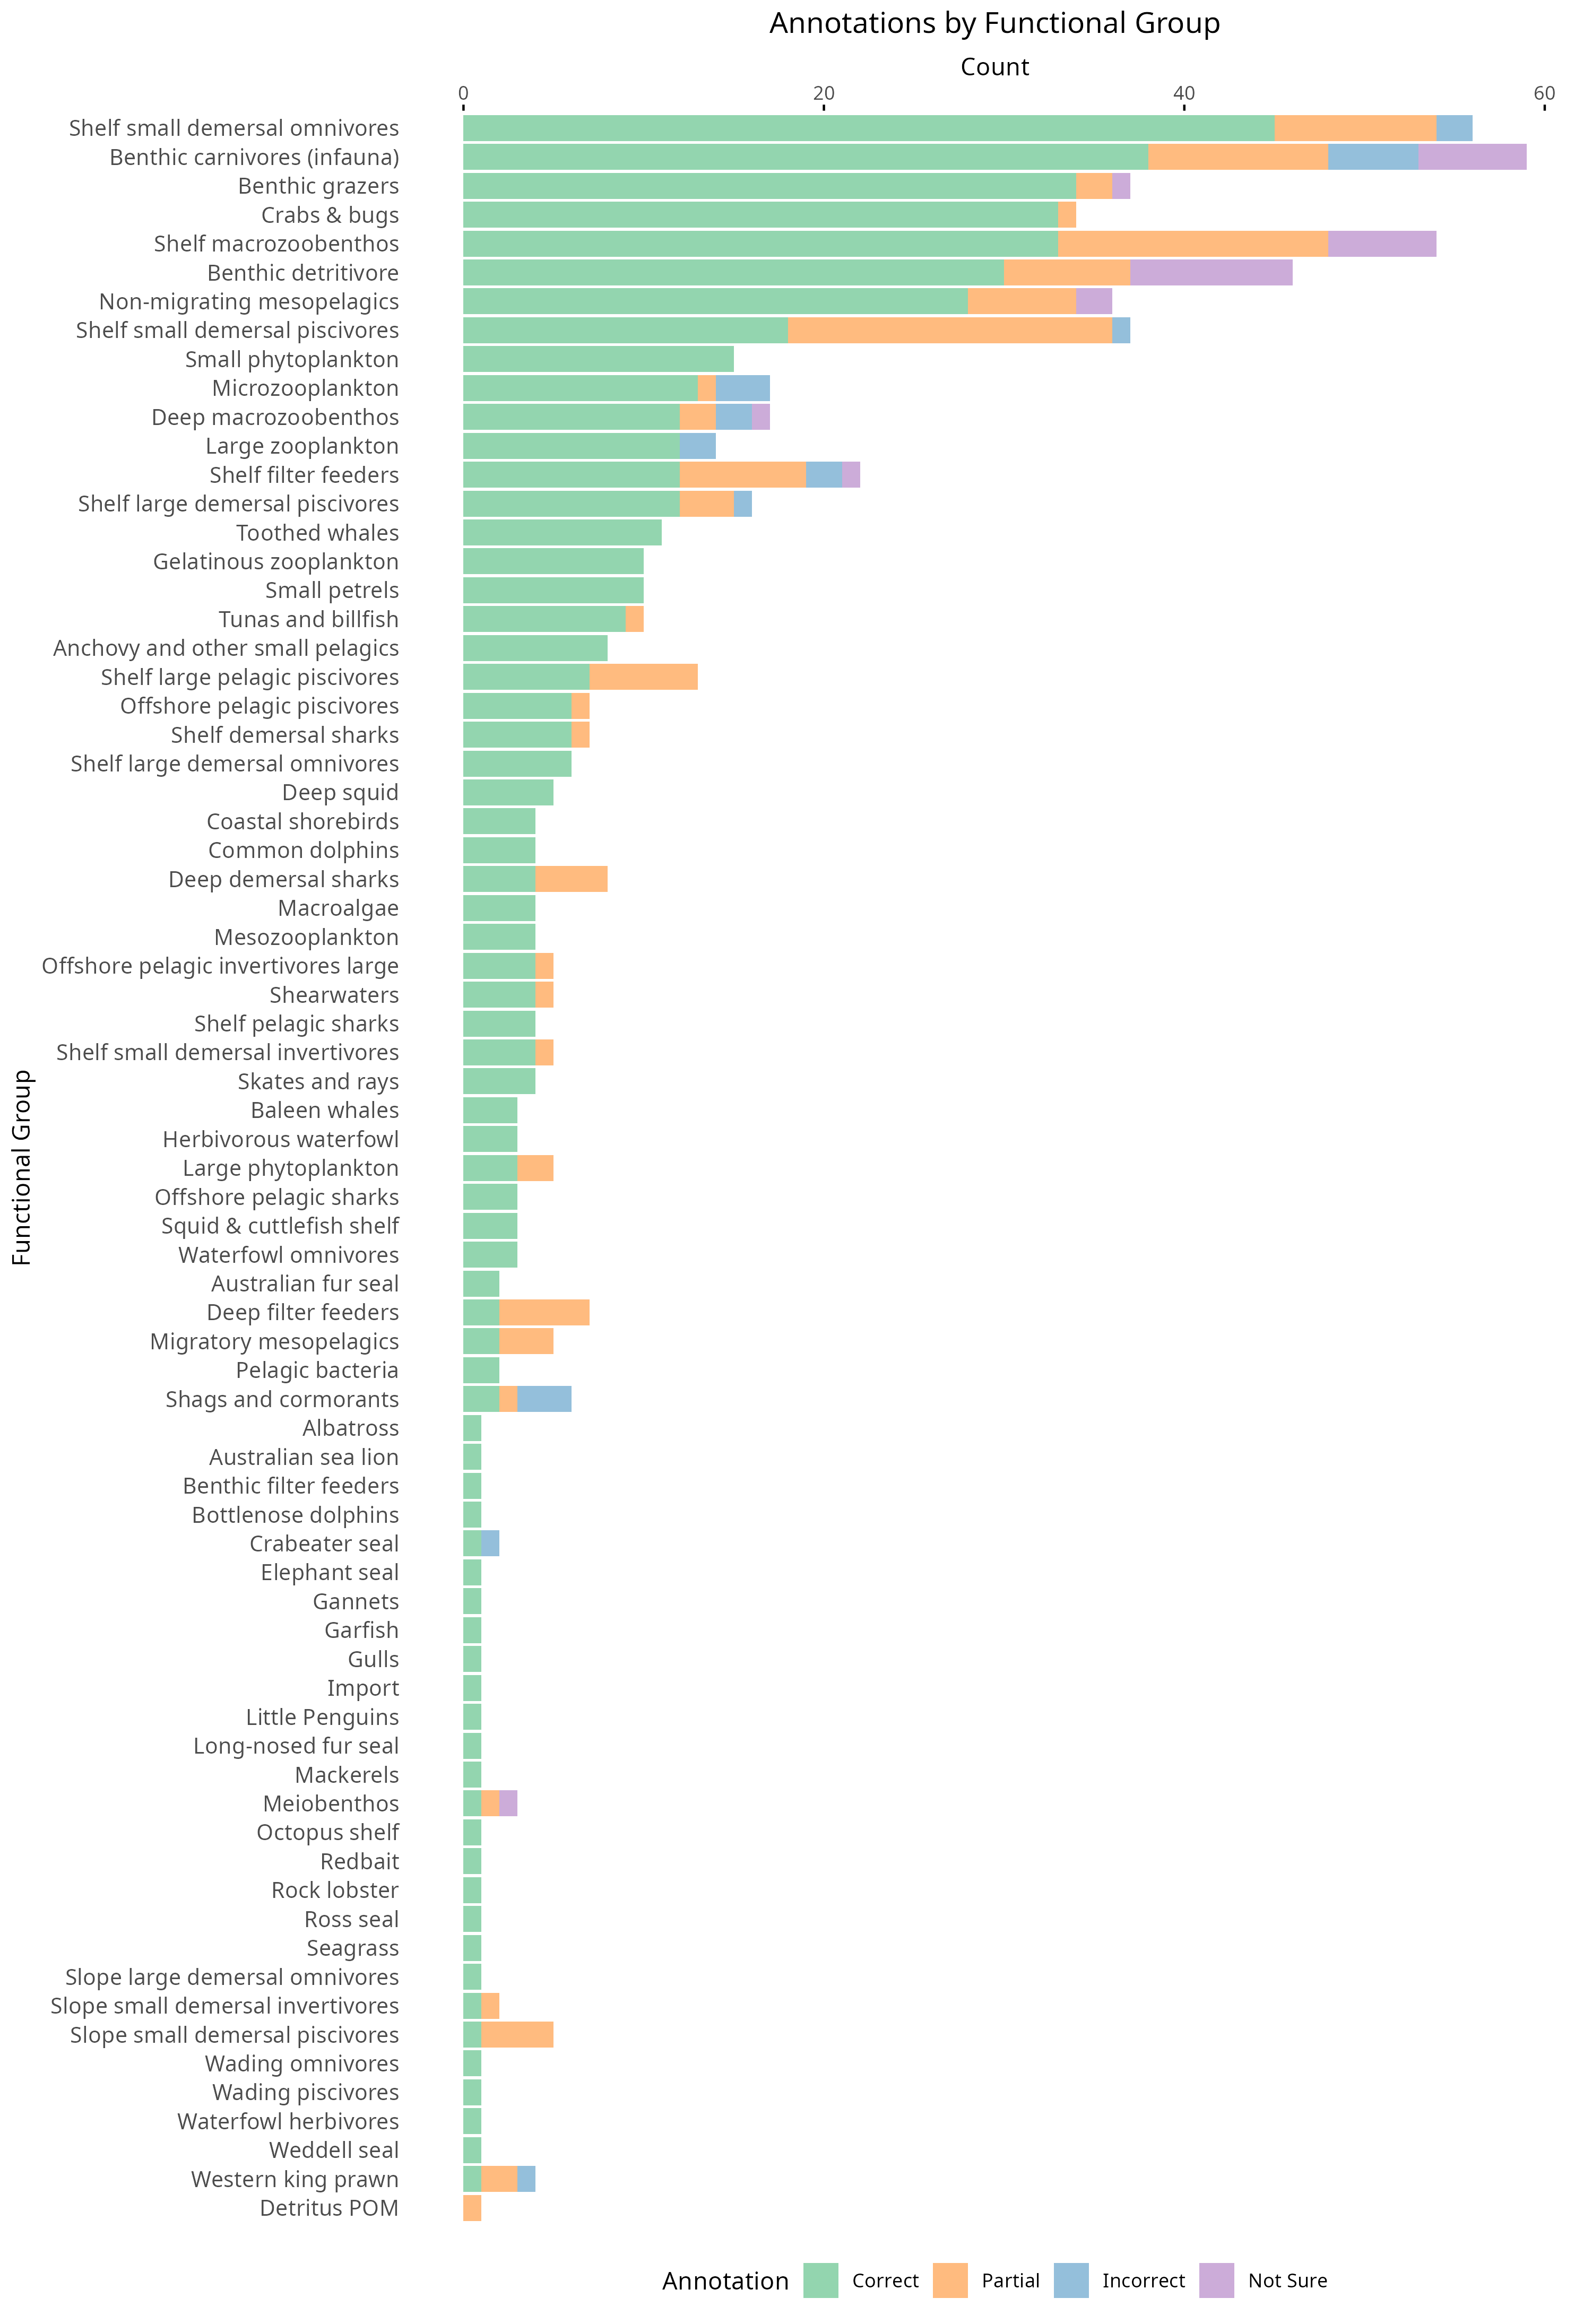
\includegraphics[width=\textwidth]{results/group_accuracy/results/annotations_by_functional_group.png}
    \caption{Accuracy of AI-assigned taxonomic groupings by functional group. The chart shows the percentage of correct (green), partial (orange), incorrect (blue), and uncertain (purple) assignments for each functional group.}
    \label{fig:annotations_by_functional_group}
\end{figure}

\begin{landscape}
\begin{figure}[htbp]
    \centering
    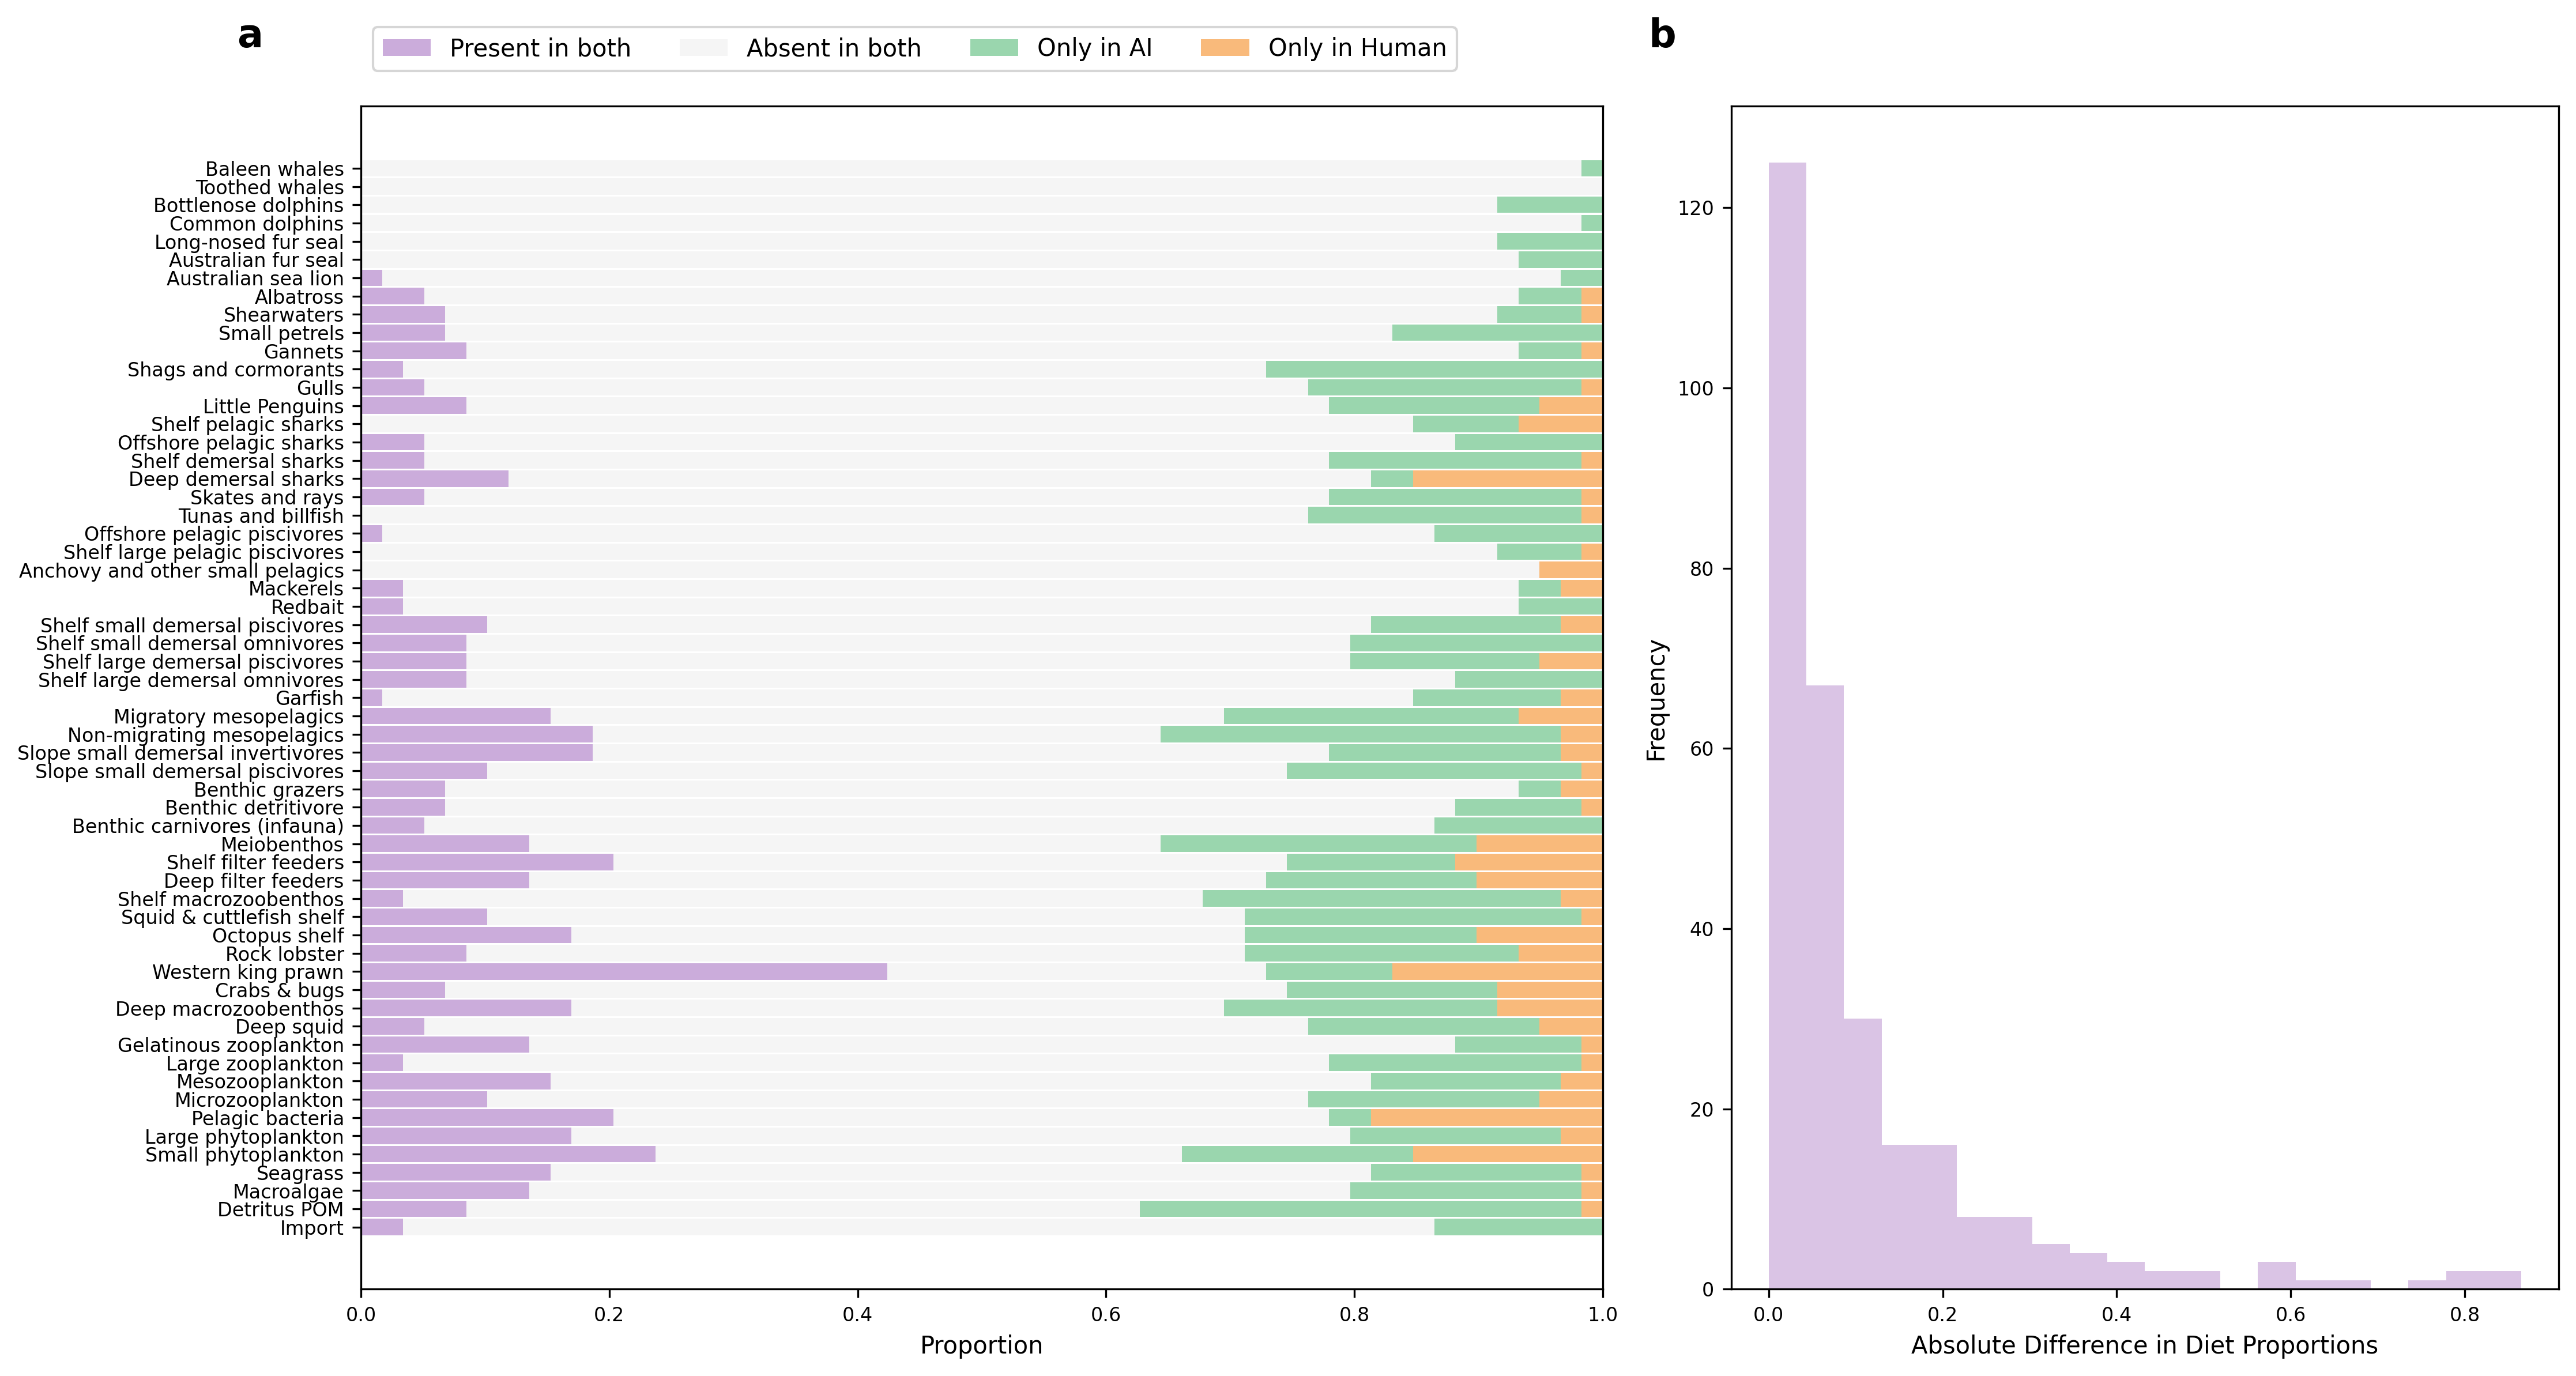
\includegraphics[width=1.2\paperwidth]{figures/diet_matrix_validation/simplified_comparison.png}
    \caption{Comparison of expert-created and AI-generated diet matrices for the Great Australian Bight ecosystem. (a) Presence-absence patterns showing the proportion of different interaction types across functional groups. Dark purple indicates interactions present in both matrices, orange shows expert-only interactions, teal shows AI-only interactions, and light grey indicates absence in both. (b) Distribution of absolute differences in diet proportions where both matrices indicate an interaction, showing the frequency of different magnitudes of disagreement between AI and expert estimates.}
    \label{fig:gab_comparison}
\end{figure}
\end{landscape}

\subsection{Framework Implementation and Performance}
% Addressing Objective 1: Present a systematic, AI-assisted framework for assembling and parameterizing EwE diet matrices

\subsubsection{Scale and Processing Efficiency}
We evaluated our framework through five independent runs across three distinct Australian regions, processing a total of 39,722 species. The framework handled 10,621 species in the Northern Australia's tropical reef ecosystem, 17,068 in the South East shelf's coastal and pelagic environments, and 12,033 in the South East Offshore's deep-water systems. 

\subsubsection{Computational Efficiency}
The computational requirements of the AI framework varied across regions. Total processing time ranged from 2.8 to 4.8 hours across regions. The most time-intensive stage was the downloading of biological data from online databases, accounting for approximately 70\% of the total processing time. Species identification typically required 0.01 hours, while the AI-driven species grouping process averaged 0.26 hours. Diet data collection and matrix construction required 0.7 and 0.04 hours respectively, with final parameter estimation taking 0.20 hours. On average, the framework required 0.7 seconds per species for data downloading and 0.2 seconds per species for diet data collection, though these rates varied considerably between regions due to differences in data availability and species complexity.
\begin{table}[htbp]
\centering
\footnotesize
\caption{Computational requirements by region and processing stage}
\label{tab:timing_analysis}
\begin{tabular}{lccccccc}
\hline
Region & Species & \multicolumn{6}{c}{Processing Time (hours)} \\
\cline{3-8}
 & Count & Identification & Data & Grouping & Diet & Matrix & Parameter \\
 & & & Download & & Collection & Construction & Estimation \\
\hline
v2 NorthernTerritory & 11,362 & 0.01 & 2.2 & 0.2 & 0.2 & 0.04 & 0.2 \\
v2 SouthEastInshore & 13,901 & 0.01 & 2.8 & 0.2 & 1.6 & 0.04 & 0.2 \\
v2 SouthEastOffshore & 15,821 & 0.01 & 3.3 & 0.4 & 0.3 & 0.04 & --- \\
\hline
\end{tabular}
\vspace{1ex}
\end{table}



\section{Discussion}

\subsection{Validation Assessment}

Our validation tests reveal both strengths and limitations in the framework's ability to construct reliable ecosystem models. The framework demonstrates strong internal consistency, with high stability scores (98.8-99.6\%) in species classifications across regions and robust correlations in predator-prey rankings ($\rho = 0.72-0.89$). This consistency suggests the framework makes systematic rather than arbitrary decisions in constructing ecological relationships. However, these metrics must be interpreted cautiously, as they reflect the framework's reproducibility rather than ecological accuracy.

The Great Australian Bight comparison against expert knowledge provides important insights into the framework's reliability. The high success rate in identifying absent trophic interactions (73.1\%) indicates the framework effectively avoids spurious ecological connections. However, the moderate correlation (0.385) with expert-assigned diet proportions and the tendency to miss specialised ecological groups reveals important limitations. The framework shows a bias toward generalised classifications that may overlook management-relevant distinctions, particularly when it comes to accommodating functional groups that are comprised of only a single species. 

The framework's handling of ecological complexity shows mixed results. While it successfully captures broad trophic patterns and adapts to regional differences, its treatment of species that span multiple functional roles needs improvement. For instance, the variable classification of anemones and flatfishes between functional groups, while partially reflecting natural ecological flexibility, suggests the need for more nuanced classification approaches. The identification of additional trophic interactions not present in expert matrices (14.5\%) requires careful evaluation - these could represent either over-connection or potentially valid relationships that merit further investigation.

These validation outcomes suggest the framework can serve as a useful starting point for ecosystem model development, particularly in its ability to avoid implausible ecological connections and maintain consistent broad-scale trophic structures. However, its outputs require expert review, especially for specialised ecological groups and complex trophic relationships. The balance between the framework's systematic approach and the need for ecological expertise emerges as a key consideration for its practical application.

\subsection{Applications for EBFM}

Given the validation outcomes, the framework shows promise as a rapid prototyping tool for ecosystem-based fisheries management. Its demonstrated ability to avoid spurious ecological connections while maintaining consistent broad-scale trophic structures makes it valuable for initial model development, reducing construction time from months to hours, with total processing times ranging from 2.6 to 4.9 hours per region. However, the framework's limitations with specialised groups and single-species functional units means it should be used as a starting point for expert refinement rather than a standalone solution.

The framework's systematic approach to uncertainty quantification helps identify where additional data collection or expert input is most needed. For instance, its higher performance in identifying absent interactions versus capturing expert-identified relationships suggests where manual review should focus. This aligns with recent approaches to uncertainty-aware ecosystem management, while the framework's consistent methodology across regions supports standardised approaches to model development across jurisdictions.

\subsection{Limitations and Uncertainties}

Our validation results highlight three key limitations of the framework. First, the framework's bias toward generalised classifications, evidenced by its difficulty with single-species functional groups in the GAB comparison, reflects fundamental limitations in how the AI system processes ecological relationships. 

Second, the framework's reliance on Claude 3.5 Sonnet, a closed-source large language model, introduces scientific reproducibility challenges. While our validation demonstrates consistent performance, we cannot fully examine the model's decision-making process or potential biases. This ``black box'' nature, as discussed by \cite{Fernandes2024}, particularly affects our ability to understand why the framework sometimes deviates from expert-derived classifications.

Third, practical implementation faces computational and data-related constraints. Data harvesting operations proved time-intensive, and the framework's performance varied with data availability across regions and ecological roles. These technical barriers, combined with the need for ecological expertise to validate outputs, create implementation challenges similar to those identified by \cite{Fernandes2024} in other AI-based ecological applications. Future iterations might benefit from exploring open-source alternatives \citep{Kommineni2024} and developing more transparent decision-making processes.

\subsection{Future Development and Assessment}

To address the identified limitations, several key areas require further development. First, the framework's handling of specialised ecological groups needs improvement, particularly for commercially important single-species units. This could involve developing specific protocols for identifying and preserving management-relevant distinctions during the classification process. Second, to enhance scientific reproducibility, future versions should explore the capability of other LLMs, including open-source LLMs which can be more transparently assessed than proprietary models like Claude.

Third, systematic validation across diverse ecosystem types is needed to establish operational boundaries. This should include testing in both data-rich temperate systems and data-sparse tropical environments, with particular attention to how the framework handles specialised ecological roles in different contexts. Throughout this development, the framework should maintain its role as a collaborative tool that complements rather than replaces expert judgment, focusing on rapid prototyping while preserving the critical role of ecological expertise in model refinement.

Fourth, we rely heavily on online databases which are subject to data quality issues and biases. Future work should explore how to incorporate local knowledge and expert judgment into the framework to address these limitations. This could involve developing more sophisticated data integration methods that combine structured data from online sources with unstructured local knowledge, as well as exploring how to incorporate expert feedback into the AI decision-making process.

Finally, the framework's utility for ecosystem-based fisheries management should be further explored through case studies that evaluate its effectiveness in building models that support management decisions. This could involve comparing the performance of models built using the framework to those built using traditional methods, as well as assessing the framework's ability to support management-relevant analyses such as scenario testing and policy evaluation.

\subsection{Conclusion}

While we have shown some initial promising results in terms of the framework's ability to produce replicable diet matrices that share qualities with those used by expert human modellers, further assessment by experienced ecologists and EwE modellers is needed to evaluate the ecological soundness and utility of the produced groupings and diet matrices. The framework's diet proportion estimates should be compared against expert knowledge, focusing on both common and rare trophic relationships. These evaluations would establish clear boundaries for the framework's operational use in ecosystem modelling.

We encourage ecologists to experiment with the framework as a collaborative tool rather than a replacement for expert judgment. The framework can rapidly generate initial model structures for expert review, enabling efficient iteration between computational suggestions and ecological expertise. Systematic testing across different ecosystem types, from data-rich temperate systems to data-sparse tropical environments, would establish the framework's utility across diverse ecological contexts. This collaborative approach would strengthen the bridge between artificial intelligence and ecological expertise in ecosystem modelling.


\section*{Acknowledgements}
SS was funded by a CSIRO R+ Postdoctoral Fellowship.

\section*{Data Availability}
The complete codebase, including all scripts, configuration files, and analysis tools, is available at [GitHub repository URL]. The validation framework, including reference group definitions and classification rules, is documented in the project repository to ensure reproducibility.

\section*{Author Contributions}
SS: Conceptualization, Methodology, Software, Validation, Formal analysis, Investigation, Resources, Data Curation, Writing - Original Draft, Writing - Review \& Editing, Visualization, Project administration. BF: Validation, Writing - Review \& Editing, Supervision, Funding acquisition. FB: Methodology, Software, Validation, Writing - Review \& Editing, Supervision. CB: Investigation, Data Curation, Validation, Writing - Review \& Editing. JS: Conceptualization, Validation, Investigation, Writing - Review \& Editing. RT: Methodology, Software, Validation, Investigation, Writing - Review \& Editing, Supervision, Funding acquisition.

\section*{Statement on the Use of Generative AI}
Generative AI tools, specifically Claude Sonnet 3.5, were utilized in the preparation of this manuscript to assist with tasks such as language refinement, text structuring, and summarization. All scientific content, data interpretation, and conclusions were independently developed and verified by the authors to ensure accuracy and integrity.

\bibliographystyle{apalike}
\bibliography{references}

\clearpage
\section*{Supplementary Material}

% Create new counter for supplement sections
\newcounter{suppsection}
\newcounter{suppsubsection}[suppsection]

% Configure supplement numbering
\renewcommand{\thesuppsection}{S\arabic{suppsection}}
\renewcommand{\thesuppsubsection}{\thesuppsection.\arabic{suppsubsection}}

% Reset counters for supplement
\setcounter{table}{0}
\setcounter{figure}{0}

% Configure table and figure numbering
\renewcommand{\thetable}{S\arabic{table}}
\renewcommand{\thefigure}{S\arabic{figure}}

% Reset and configure page numbering
\setcounter{page}{1}
\renewcommand{\thepage}{S\arabic{page}}

% Define supplement section command
\newcommand{\suppsection}[1]{%
  \refstepcounter{suppsection}%
  \section*{S\arabic{suppsection}. #1}\label{supp:\arabic{suppsection}}%
}

% Define supplement subsection command
\newcommand{\suppsubsection}[1]{%
  \refstepcounter{suppsubsection}%
  \subsection*{S\arabic{suppsection}.\arabic{suppsubsection}. #1}\label{supp:\arabic{suppsection}.\arabic{suppsubsection}}%
}

\suppsection{Data Harvesting Implementation}\label{supp:data_harvesting}

Our data harvesting system employs DuckDB for efficient querying of PARQUET files, enabling complex joins and aggregations without full memory loading. For species matching across databases, we use structured SQL queries that join on concatenated genus and species names:

\begin{verbatim}
SELECT 
    SpecCode, PreySpecCode, AlphaCode, 
    Foodgroup, Foodname, PreyStage, PredatorStage, FoodI, FoodII, FoodIII, 
    Commoness, CommonessII, PreyTroph, PreySeTroph
FROM sealifebase_df
WHERE SpecCode IN ({','.join(map(str, valid_codes))})
AND (PreyStage LIKE '%adult%' OR PreyStage LIKE '%juv%')
AND (PredatorStage LIKE '%adult%' OR PredatorStage LIKE '%juv%')
\end{verbatim}

When combining interaction data from GLOBI with diet information, we implement a comprehensive interaction mapping system that creates bidirectional records:

\begin{verbatim}
interaction_data[source_group]['preys_on'][target_group] = count
interaction_data[target_group]['is_preyed_on_by'][source_group] = count
\end{verbatim}

Our data cleaning protocol standardises types by converting numerical values to consistent formats and timestamps to ISO format. We handle null values by removing empty values, `NA' strings, and null entries while preserving data structure. Source tracking maintains database origin information for all data points.

The system implements file locking mechanisms for concurrent access, with separate locks for species data and interaction networks. We use exponential backoff retry logic for API interactions, with configurable parameters including maximum retries (5), initial delay (1 second), and maximum delay (60 seconds).

The completion check system verifies the presence of required fields including:
\begin{itemize}
\item Complete taxonomic hierarchy
\item Species-specific database records (when available)
\item Interaction data
\item Source attribution
\item Data quality indicators
\end{itemize}

The final JSON output maintains a consistent structure across all species entries, facilitating automated processing in subsequent framework stages.

\suppsection{Diet Matrix Analysis}\label{supp:diet_matrix}


\begin{landscape}
  \begin{figure}[p]
      \centering
      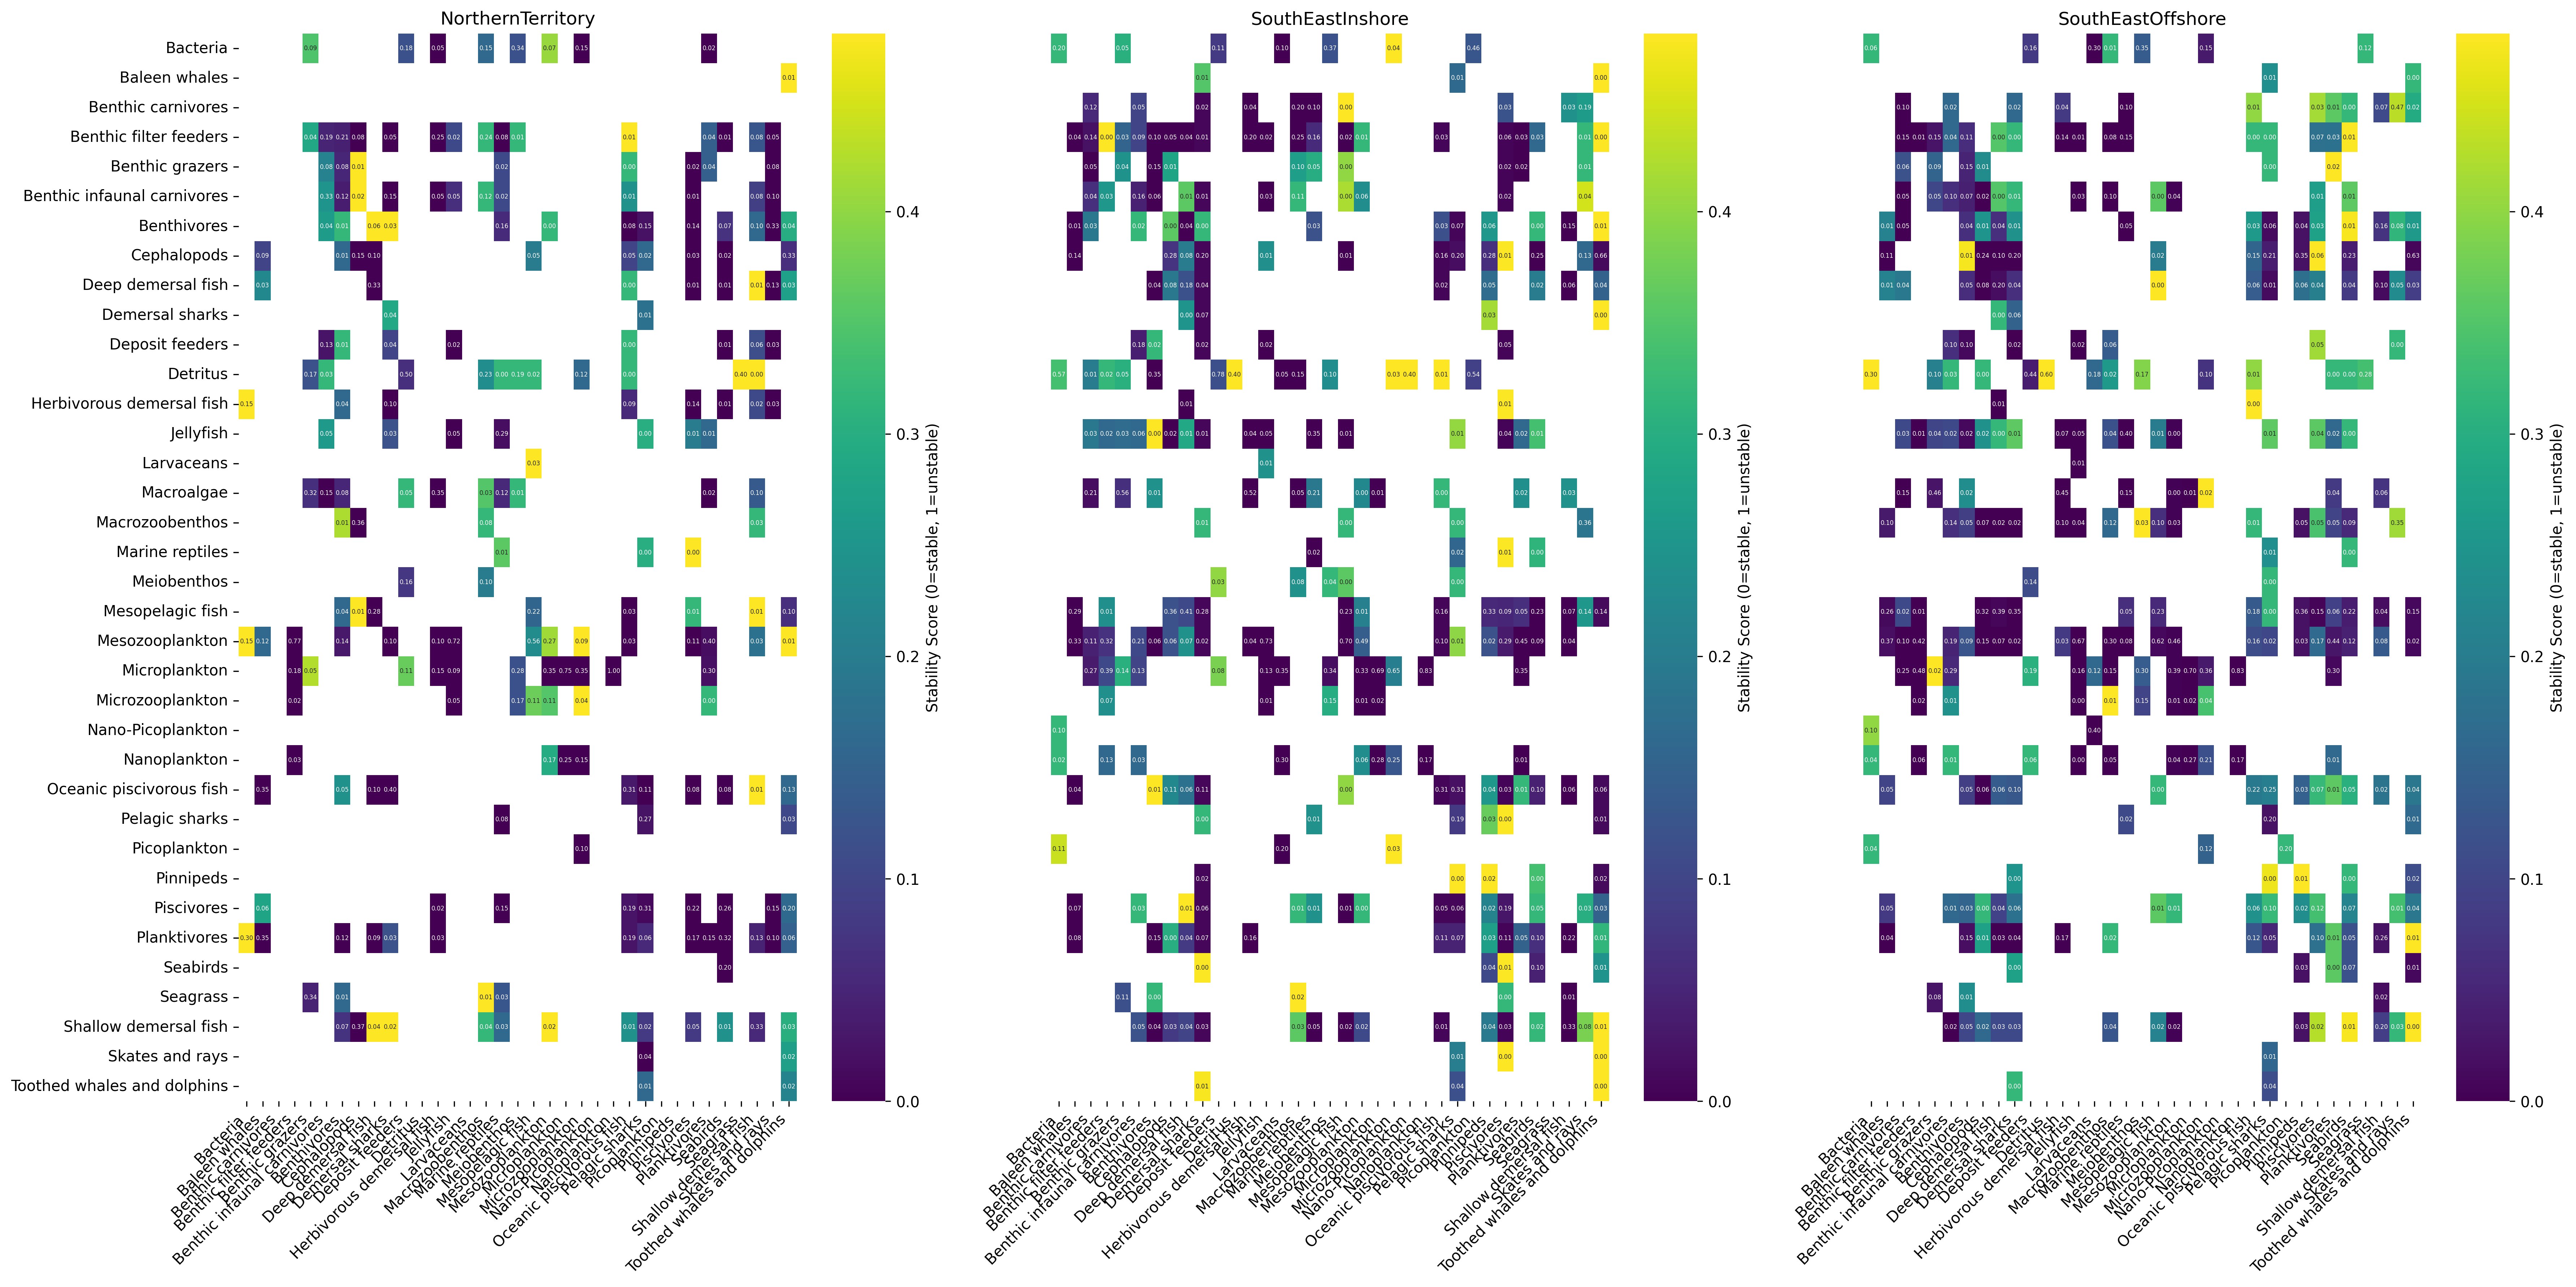
\includegraphics[width=\linewidth]{figures/diet_interaction_heatmap.png}
      \caption{Detailed diet matrix consistency across five iterations for each geographic region. Column names represent predator groups and row names represent their prey groups. Numbers in each cell indicate the mean diet proportions across five iterations, while cell colors indicate the stability score (0-1, where 0 represents perfect stability and 1 represents maximum variation). White cells represent absent feeding relationships. This comprehensive visualization complements the stability score distributions and predator-specific analyses presented in the main text (Figures 4 and 5).}
      \label{fig:diet_matrix_supp}
  \end{figure}
  \end{landscape}

\begin{landscape}
  \begin{figure}[p]
      \centering
      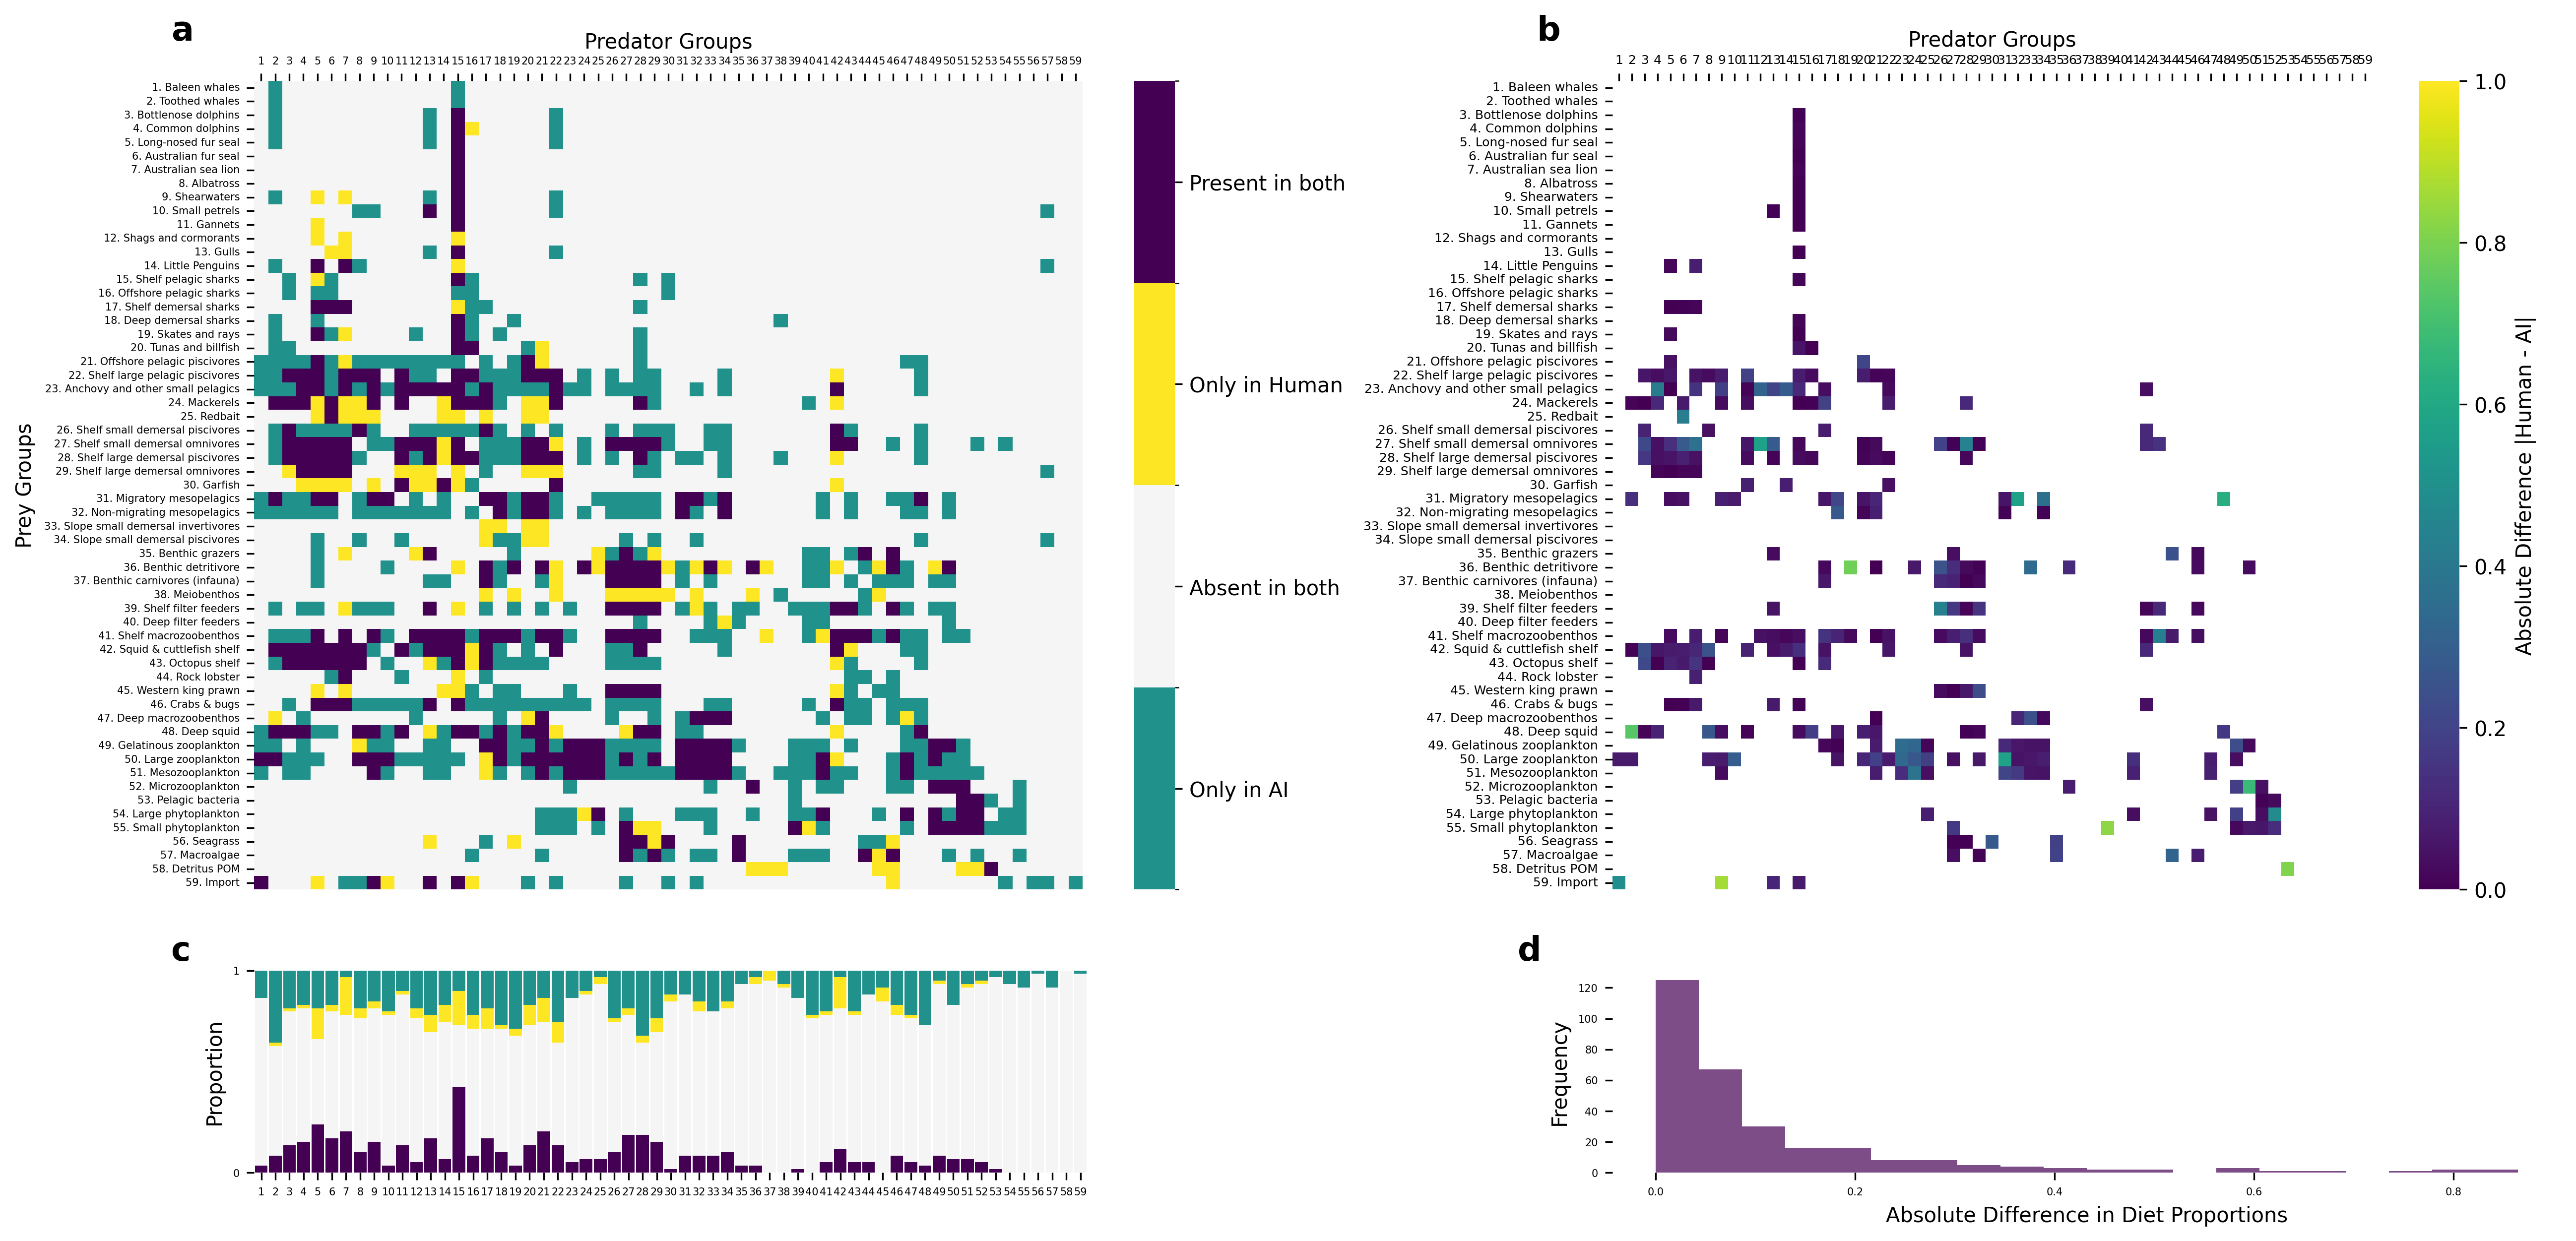
\includegraphics[width=\linewidth]{figures/diet_matrix_validation/detailed_comparison.png}
      \caption{Detailed comparison of diet matrix elements between expert-derived and AI-generated matrices for the Great Australian Bight ecosystem. Panel (a) shows the complete diet matrix with color-coded interaction types: dark purple indicates interactions present in both matrices, yellow shows expert-only interactions, teal shows AI-only interactions, and light grey indicates absence in both. Panel (b) displays the absolute differences in diet proportions between expert and AI matrices where interactions are present in both, with colors ranging from purple (small differences) to yellow (large differences). Panel (c) shows the proportional breakdown of interaction types for each predator group, while panel (d) presents the frequency distribution of absolute differences in diet proportions. This comprehensive visualization expands on Figure \ref{fig:gab_comparison} from the main text by providing a detailed view of each predator-prey relationship and quantifying the differences between expert and AI assessments.}
      \label{fig:detailed_comparison_supp}
  \end{figure}
\end{landscape}
  
\suppsection{Group Stability Analysis}\label{supp:group_stability}

\begin{figure}[htbp]
    \centering
    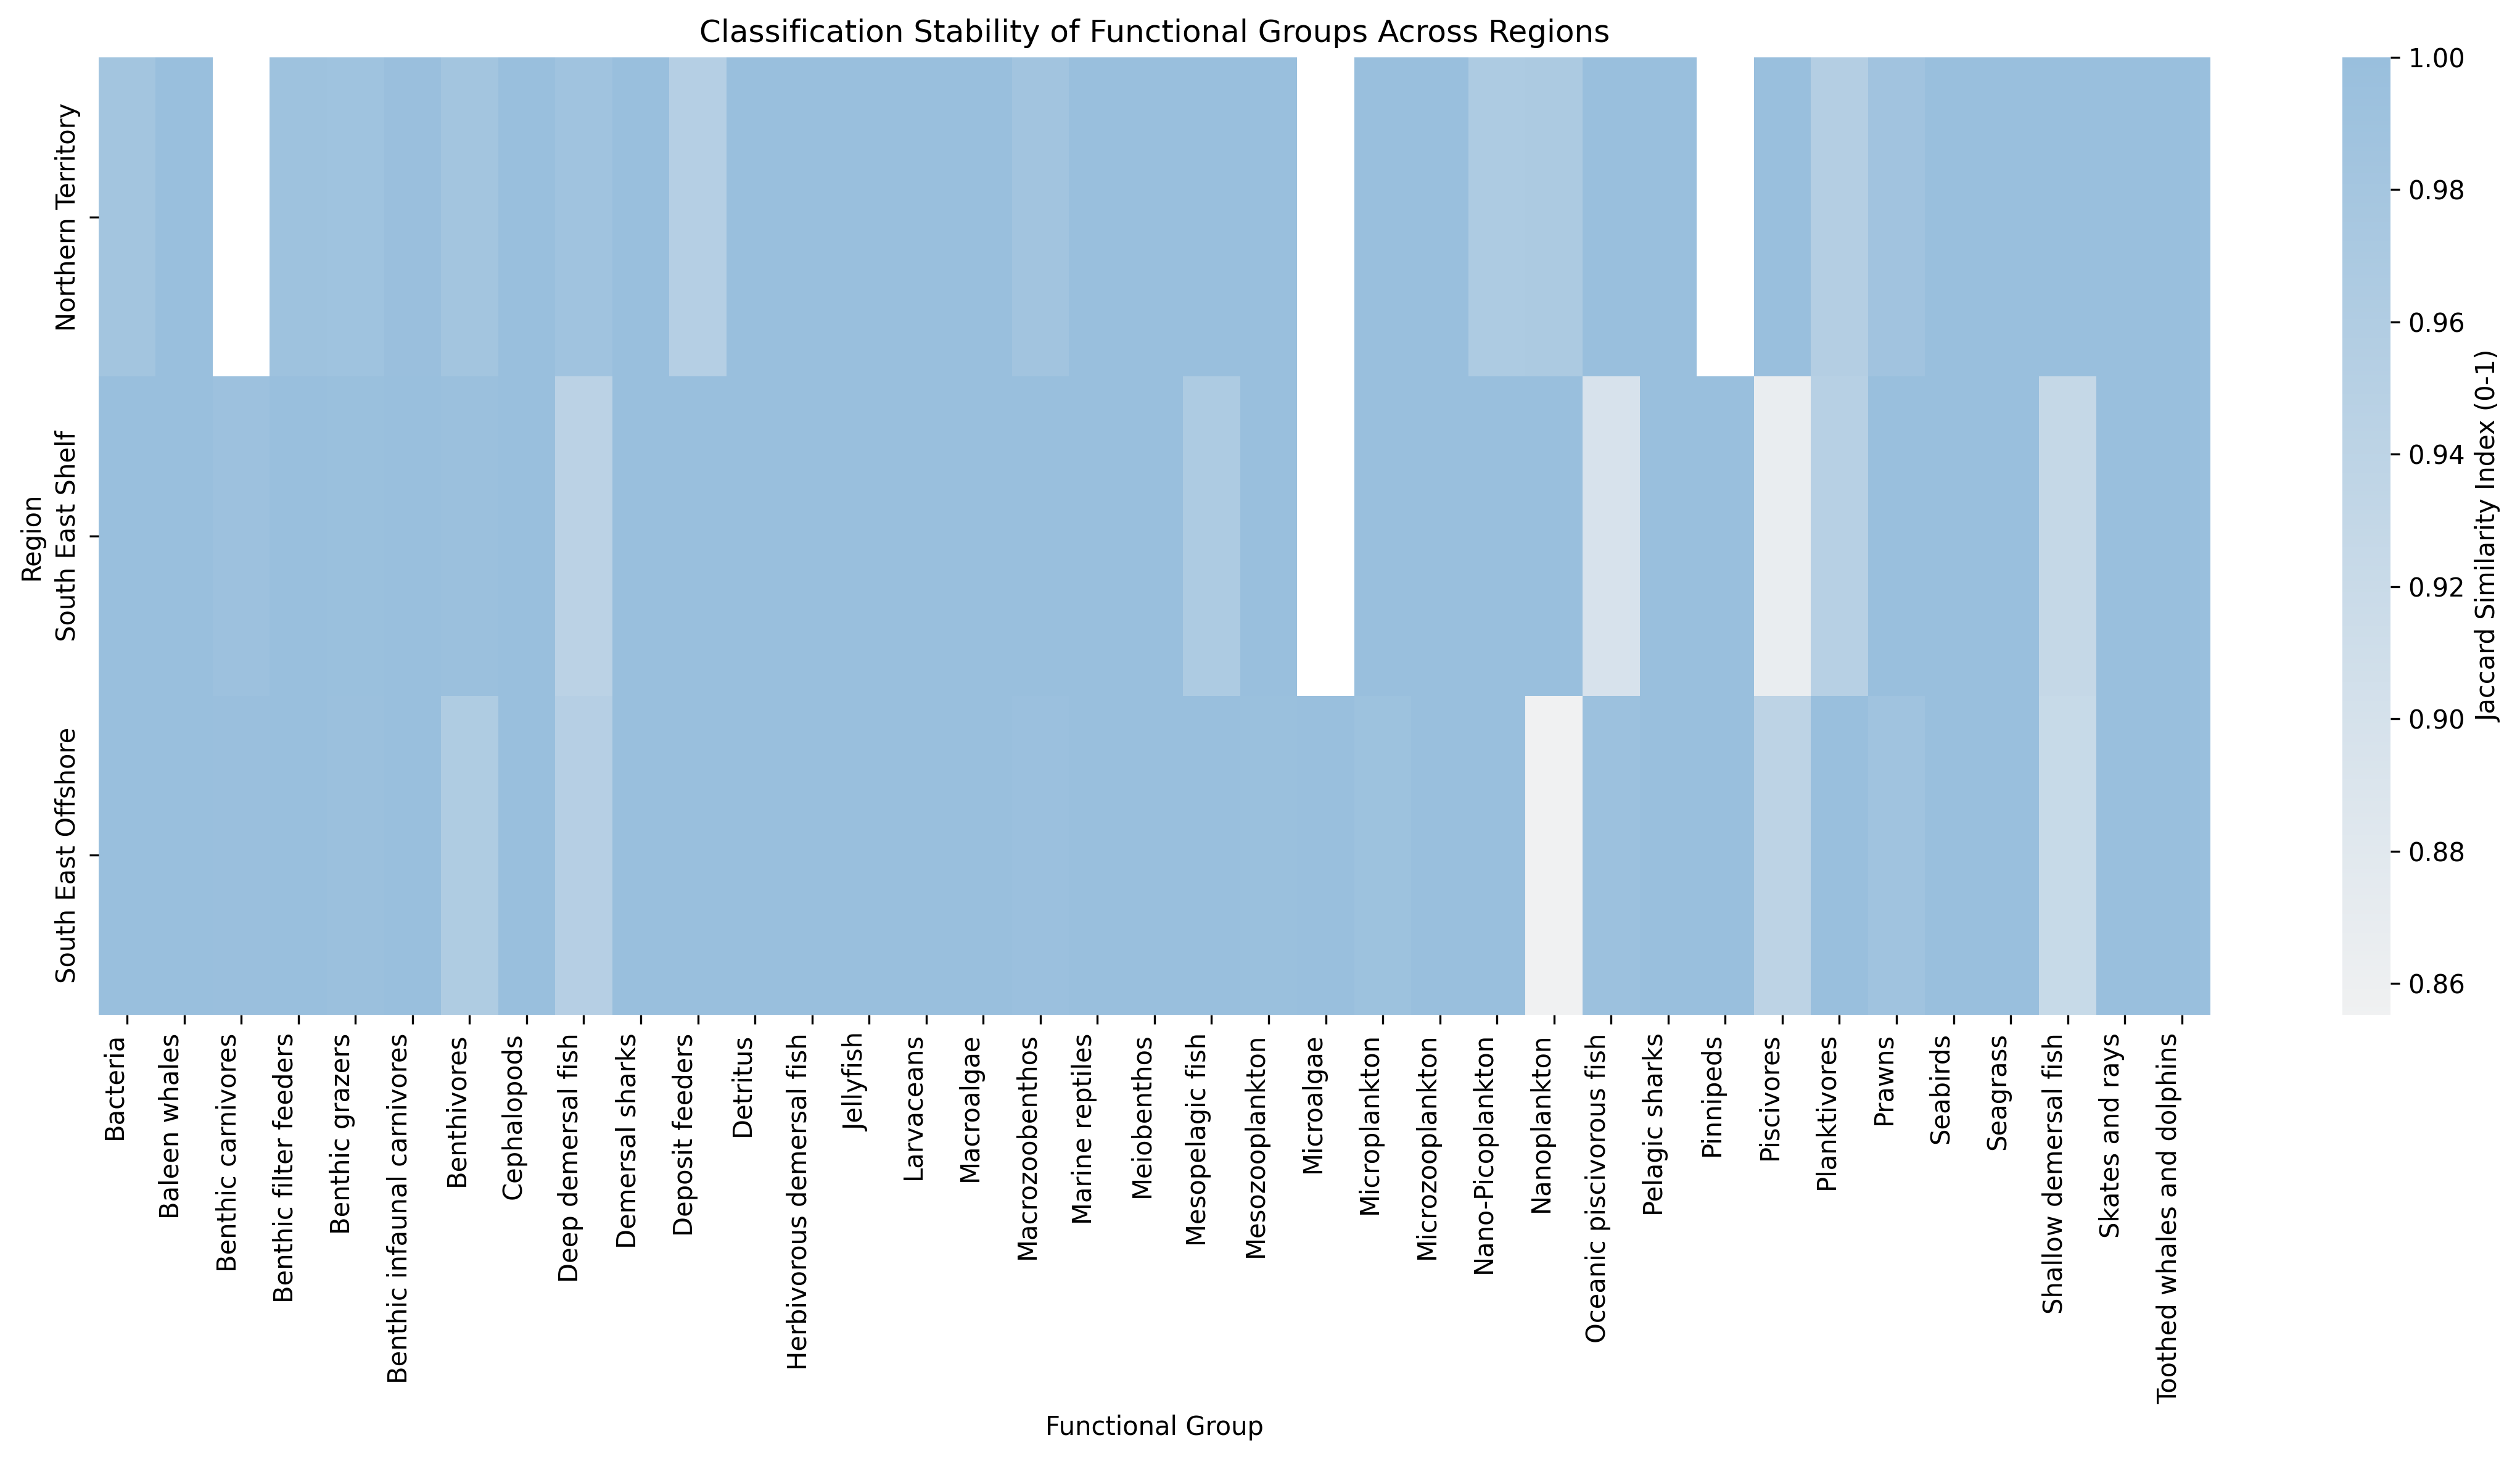
\includegraphics[width=\textwidth]{figures/group_stability_heatmap.png}
    \caption{Heatmap showing the stability of functional group classifications across regions. Each cell displays the Jaccard similarity score (ranging from 0.975 to 1.000) between consecutive framework iterations, where 1.000 indicates perfect consistency in species assignments. Yellow colors represent higher stability (scores near 1.000), while darker purple colors indicate more variable classifications (scores closer to 0.975). Most functional groups show high stability (>0.99) across all regions, with occasional variations in groups like benthic grazers and deposit feeders, particularly in the Northern Territory region. White indicates groups that were not assigned by the AI system for that region.}
    \label{fig:stability_heatmap_supp}
\end{figure}

\begin{figure}[htbp]
  \centering
  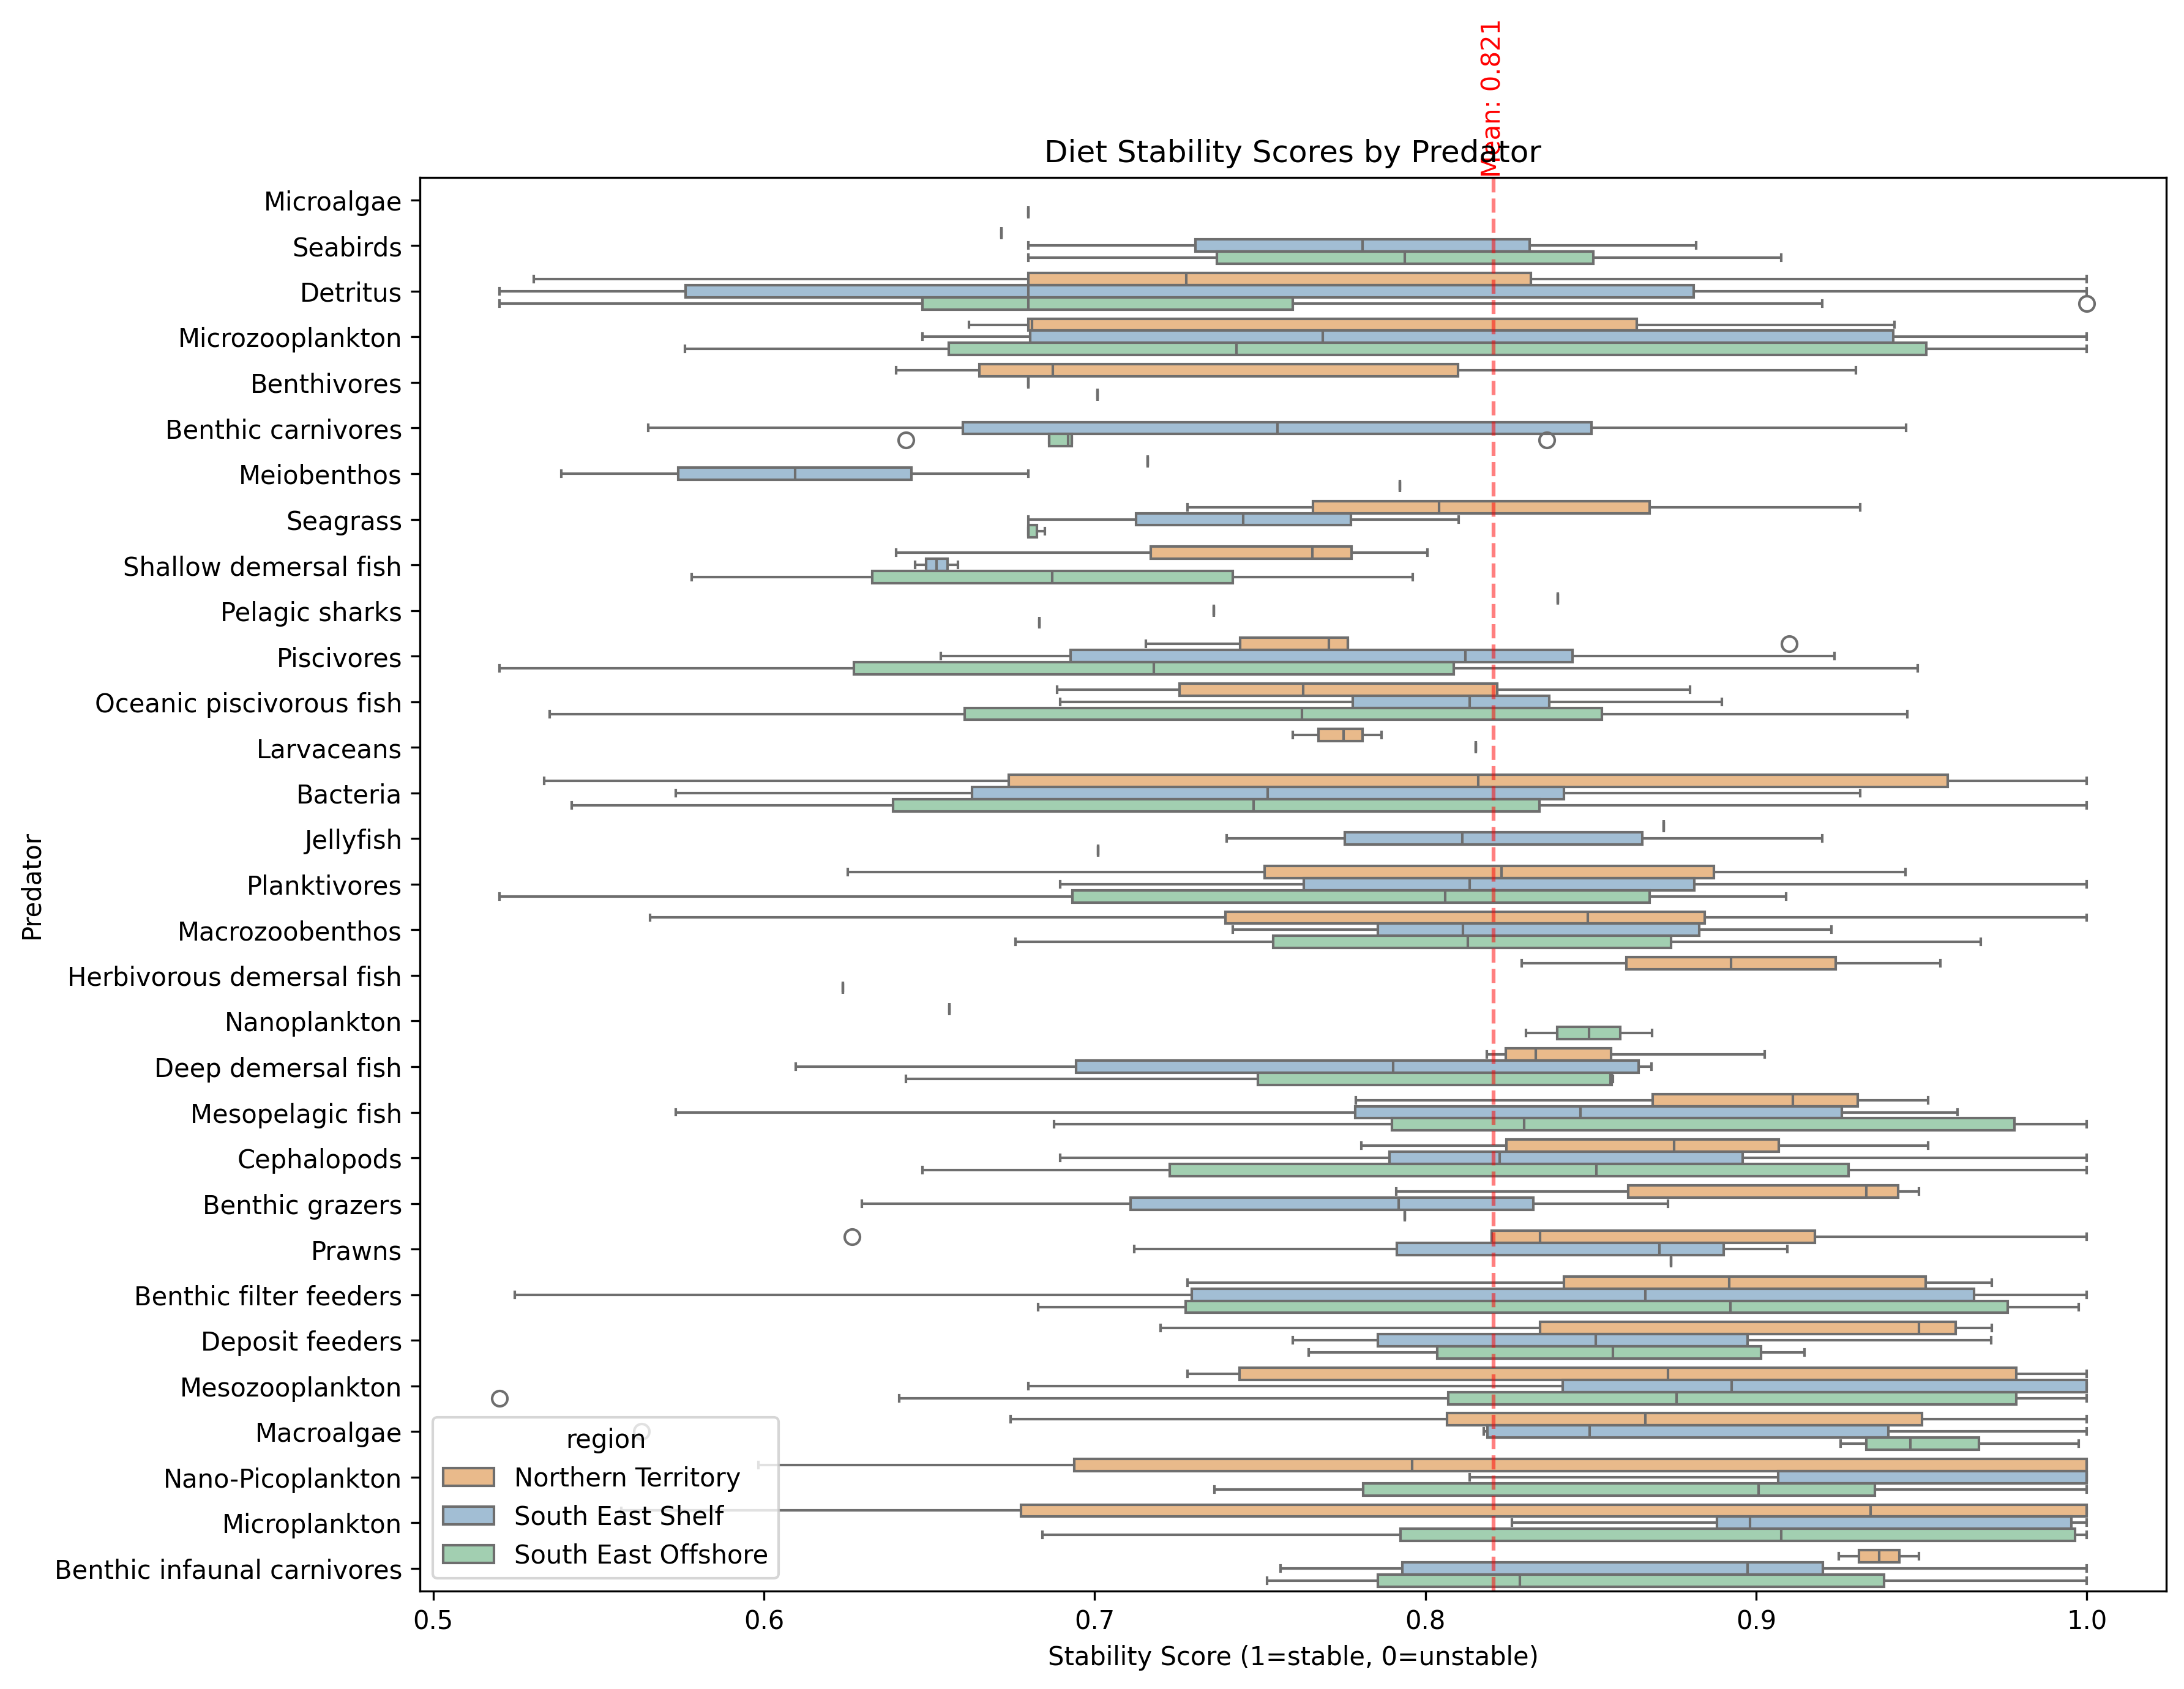
\includegraphics[width=\textwidth]{figures/predator_stability_boxplots.png}
  \caption{Diet stability scores grouped by predator, ordered by median stability. Box plots show the distribution of stability scores for each predator's diet across regions (colored by region). The red dashed line indicates the mean stability score across all predator-prey interactions. Higher scores indicate more consistent diet compositions across framework iterations.}
  \label{fig:predator_stability}
\end{figure}



\suppsection{Technical Implementation}\label{supp:technical_implementation}
  \suppsubsection{Default Grouping with Descriptions}
  
  Table \ref{tab:functional_groups} presents the complete template of potential functional groups used by the system. This template serves as a reference for group classification, though the system can create new groups or modify existing ones based on specific ecosystem characteristics.
  
  \begin{longtable}{p{0.3\textwidth}p{0.7\textwidth}}
  \caption{Complete Functional Group Template\label{tab:functional_groups}} \\
  \hline
  \textbf{Group Name} & \textbf{Description} \\
  \hline
  \endfirsthead
  \multicolumn{2}{c}{{\tablename} \thetable{} -- Continued} \\
  \hline
  \textbf{Group Name} & \textbf{Description} \\
  \hline
  \endhead
  \hline
  \multicolumn{2}{r}{{Continued on next page}} \\
  \endfoot
  \hline
  \endlastfoot
  Skates and rays & Bottom-dwelling cartilaginous fish that play a role in controlling benthic prey populations \\
  Nearshore and smaller seabirds & Small gulls, terns etc that feed near shore (possibly include penguins here too) - avian predators that link marine and terrestrial ecosystems \\
  Albatrosses & Large seabirds that forage exclusively at sea, feeding on marine prey (fishes, squids, gelatinous organisms) \\
  Skuas and giant petrels & Large predatory seabirds that feed both at sea and on land, including predation on other birds \\
  Fish-eating pinnipeds & Marine mammals (seals, sea lions) that primarily prey on fish in coastal and pelagic ecosystems \\
  Invertebrate-eating pinnipeds & Marine mammals (particularly Antarctic seals) that primarily feed on krill and other invertebrates \\
  Baleen whales & Large filter-feeding marine mammals that regulate zooplankton populations and contribute to nutrient cycling \\
  Orcas & Apex predators that uniquely prey upon other top predators including marine mammals, sharks, and large fish \\
  Sperm whales & Deep-diving cetaceans that primarily feed on deep-water squid and fish \\
  Small toothed whales and dolphins & Smaller cetaceans that primarily feed on fish and squid in surface and mid-waters \\
  Sea snakes & Marine reptiles that prey primarily on fish, particularly eels and fish eggs \\
  Crocodiles & Large predatory reptiles in coastal and estuarine waters that prey on fish, birds, and mammals \\
  Turtles & Herbivores and omnivores that breed on land \\
  Planktivores & Small fishes that feed on plankton, crucial in transferring energy from plankton to larger predators \\
  Flying fish & Epipelagic fish capable of gliding above the water surface, important prey for many predators \\
  Remoras & Fish that form commensal relationships with larger marine animals, feeding on parasites and food scraps \\
  Large oceanic piscivorous fish & Fish-eating predators in open ocean environments, mid-sized non-migratory species (e.g. barracuda) \\
  Tuna and Billfish & Large oceanic predatory fish, highly mobile, often dive to feed deeper into the water column \\
  Shelf small benthivores & Small bodied fish that feed on benthic organisms, playing a key role in benthic-pelagic coupling, live in shelf waters \\
  Shelf demersal omnivorous fish & Medium sized demersal fish that feed on invertebrates as well as smaller fish, live in shelf waters \\
  Shelf medium demersal piscivores & Medium sized demersal fish living near the bottom in shallow waters, often important in benthic food webs, feed on other fish primarily, live in shelf waters \\
  Shelf large piscivores & Fish-eating predatory fishes found in various marine habitats, important in controlling prey fish populations \\
  Herbivorous demersal fish & Bottom-associated fish that primarily feed on plants, important in controlling algal growth \\
  Slope/deep water benthivores & Small to mid sized fish that feed on benthic organisms and live on the shelf or seamounts \\
  Slope/deep demersal omnivorous fish & Medium sized demersal fish that feed on invertebrates as well as smaller fish, live in slope or seamount waters \\
  Slope/deep medium demersal piscivores & Medium sized demersal fish that feed on other fish primarily, live in slope or seamount waters \\
  Slope/deep large piscivores & Fish-eating predatory fishes found in various marine habitats in deeper water, live in slope or seamount waters \\
  Migratory mesopelagic fish & Fish living in the mesopelagic zone, undertake diel vertical migration, important in energy transfer between depths \\
  Non-migratory mesopelagic fish & Fish living in the mesopelagic zone, non-migratory species, important in energy transfer between depths \\
  Reef sharks & Top predators in coral reef ecosystems, controlling fish populations and maintaining reef health \\
  Pelagic sharks & Open-ocean predators that help regulate populations of fishes and squids \\
  Demersal sharks & Bottom-dwelling sharks, including dogfishes, that control populations of fishes and invertebrates on and near the seafloor \\
  Cephalopods & Intelligent mollusks like squid and octopus, important predators in many marine ecosystems \\
  Hard corals & Reef-building colonial animals that create complex habitat structure through calcium carbonate deposition \\
  Soft corals & Colonial animals that contribute to reef habitat complexity without building calcium carbonate structures \\
  Sea anemones & Predatory anthozoans that can form symbiotic relationships with fish and crustaceans \\
  Hydrothermal vent communities & Specialized organisms living around deep-sea vents, including chemosynthetic bacteria and associated fauna \\
  Cold seep communities & Organisms adapted to methane and sulfide-rich environments on the seafloor \\
  Deep-sea glass sponges & Filter-feeding animals that create complex deep-water habitats and are important in silicon cycling \\
  Sea cucumbers & Deposit-feeding echinoderms important in sediment processing and bioturbation \\
  Sea urchins & Herbivorous echinoderms that can control macroalgal abundance and affect reef structure \\
  Crown-of-thorns starfish & Coral-eating sea stars that can significantly impact reef health during population outbreaks \\
  Benthic filter feeders & Bottom-dwelling organisms that filter water for food, important in nutrient cycling and regulating water quality in various depths - bivalves, crinoids, sponges \\
  Macrozoobenthos & Mobile large bottom-dwelling invertebrates in both shallow and deep waters, important in benthic food webs and bioturbation (predatory or omnivorous) \\
  Benthic grazers & Bottom-dwelling organisms that graze on algae and detritus, influencing benthic community structure \\
  Prawns & Small crustaceans that are important in benthic and pelagic food webs \\
  Meiobenthos & Tiny bottom-dwelling organisms, important in sediment processes and as food for larger animals \\
  Deposit feeders & Animals that feed on organic matter in sediments, important in nutrient cycling \\
  Benthic infaunal carnivores & Predatory animals living within the seafloor sediments \\
  Sedimentary Bacteria & Microscopic organisms crucial in nutrient cycling and the microbial loop in marine ecosystems \\
  Large carnivorous zooplankton & Fish larvae, arrow worms and other large predatory zooplankton \\
  Antarctic krill & Key species in Antarctic food webs, particularly important as prey for whales, seals, and seabirds \\
  Ice-associated algae & Microalgae living within and on the underside of sea ice, important primary producers in polar regions \\
  Ice-associated fauna & Specialized invertebrates living in association with sea ice, important in polar food webs \\
  Mesozooplankton & Medium-sized zooplankton (200 µm to 2 cm) that feed on smaller plankton and serve as food for larger animals \\
  Microzooplankton & Tiny zooplankton (20 µm to 200 µm) that graze on phytoplankton and bacteria, forming a crucial link in the microbial food web \\
  Pelagic tunicates & Including larvaceans, salps, and pyrosomes, important in marine snow formation and carbon cycling \\
  Jellyfish & Predatory gelatinous species \\
  Diatoms & Larger phytoplankton (20 µm to 200 µm), silica dependent important primary producers in marine ecosystems \\
  Dinoflagellates & Mixotrophic species (20 µm to 200 µm) that can switch between primary production and consumption as needed \\
  Nanoplankton & Plankton ranging from 2 µm to 20 µm in size, including small algae and protozoans \\
  Picoplankton & Plankton ranging from 0.2 µm to 2 µm in size, including both photosynthetic and heterotrophic organisms \\
  Microalgae (microphytobenthos) & Microscopic algae that live on the seafloor or attached to other organisms \\
  Pelagic bacteria & Watercolumn dwelling bacteria, consume marine snow amongst other things \\
  Seagrass & Marine flowering plants that form important coastal habitats and nursery areas \\
  Mangroves & Salt-tolerant trees forming critical coastal nursery habitats and protecting shorelines \\
  Salt marsh plants & Coastal vegetation adapted to periodic flooding, important in nutrient cycling and shoreline protection \\
  Macroalgae & Seaweeds of various sizes that provide habitat and food for many species, including both canopy and understory forms \\
  Symbiotic zooxanthellae & Photosynthetic dinoflagellates living within coral and other marine invertebrates \\
  Cleaner fish and shrimp & Species that remove parasites from other marine animals, important in reef health \\
  Discards & Carrion and freshly discarded material from fisheries activities \\
  Detritus & Labile components of natural death and waste \\
  \end{longtable}
  
  \suppsubsection{Retrieval-Augmented Generation Implementation}\label{supp:rag_implementation}
  
  We implement a retrieval-augmented generation system using ChromaDB for vector storage and document management. Document processing begins with LlamaParse conversion of source materials to markdown format, preserving structural elements while enabling consistent text extraction across document types. We segment documents using a token-aware chunking strategy with a 2000-token maximum size, determined through empirical testing to balance context preservation with model limitations.
  
  Document processing follows a two-phase approach. The initial phase generates embeddings for each document chunk using Azure OpenAI's text-embedding-3-small model, storing them in ChromaDB's PersistentClient. The system maintains an indexed\_files.json registry to track processed documents. The second phase handles incremental updates, identifying and processing only new content when documents are added to the source directory.
  
  For diet composition analysis, we implement a two-stage query process. The first stage employs a simple query to retrieve relevant document chunks:
  
  \begin{prompt}
  What do [group] eat?
  \end{prompt}
  
  The system embeds this query using the same Azure OpenAI model and performs vector similarity search to identify relevant document chunks. These results combine with structured data sources including species occurrence frequencies, food category classifications, and GLOBI interaction data to form a comprehensive input for the second stage.
  
  We implement comprehensive error handling throughout the pipeline. The system employs exponential backoff retry logic for API interactions, with configurable parameters including maximum retries (10), initial delay (1 second), and maximum delay (300 seconds). For model interactions, we utilise LlamaIndex's query engine with zero-temperature sampling to ensure deterministic responses. The system supports multiple language model backends including Claude-3 Sonnet (200k token context), GPT-4, and AWS Claude, enabling flexible deployment based on availability and performance requirements.
  
  The system maintains separate storage contexts for different document collections through ChromaDB's collection management. This separation prevents cross-contamination between knowledge bases while enabling efficient parallel processing. We track document citations throughout the retrieval process, maintaining provenance information for all retrieved content. The complete implementation, including embedding generation, chunking algorithms, and query processing functions, is available in the project repository.


\end{document}
\end{document}
\end{document}
